\cleardoublepage
\chapter{Data Collection}\label{sec:data}

\section{Introduction}

The output of the DAVIS camera is the main source of information. On the one hand, we have the grayscale frames @40 Hz. On the other hand, the events are generated asynchronously and are saved with their pixel location, polarity and timestamp. Therefore, some kind of representation is needed to visually inspect the data. For this purpose the events are represented using event images, where the events are accumulated for a certain time window (30 ms in our case) and a pixelwise histogram of events is built, generating a 2D image. Usually, pixels with gray color mean that no events occurred in the current time window, whereas different shades of white indicate positive polarity and shades of black indicate negative polarity. Event images have an intuitive and informative interpretation, as events are caused by moving edges, these frames are like edge maps and edges convey a lot of information of a scene. Moreover, if the object does not slip, it will not move, as its relative pose with respect to the camera does not change, thus no events will be generated due to the motion (only some events may be generated due to illumination changes) and no edges will be visible in the event images. On the contrary, if the object slips we will be able to see edges in the event images.\\

Using the experiment setup described in the previous chapter, we can start to record data of pick-and-place motions. Concretely, in ~\Cref{fig:rob_traj} we can observe a sequence of images of a complete pick-and-place motion executed by Panda with the assembled DAVIS 346. The images \textit{a-c}, show the reaching phase, where no slip needs to be detected. Specifically, in \textit{c} the gripper closes and the movement with the object starts, ending at image \textit{e}, and it is between these two instances where slip has to be detected, if it occurs. Finally, the object is released and the arm returns to the home position (\textit{f}). It is worth noticing that the relative position of the object with respect to the gripper changes significantly between image \textit{c} and images \textit{d} and \textit{e}, meaning that a slip occurred during the lifting phase.\\

\begin{figure}[h]
    \centering
    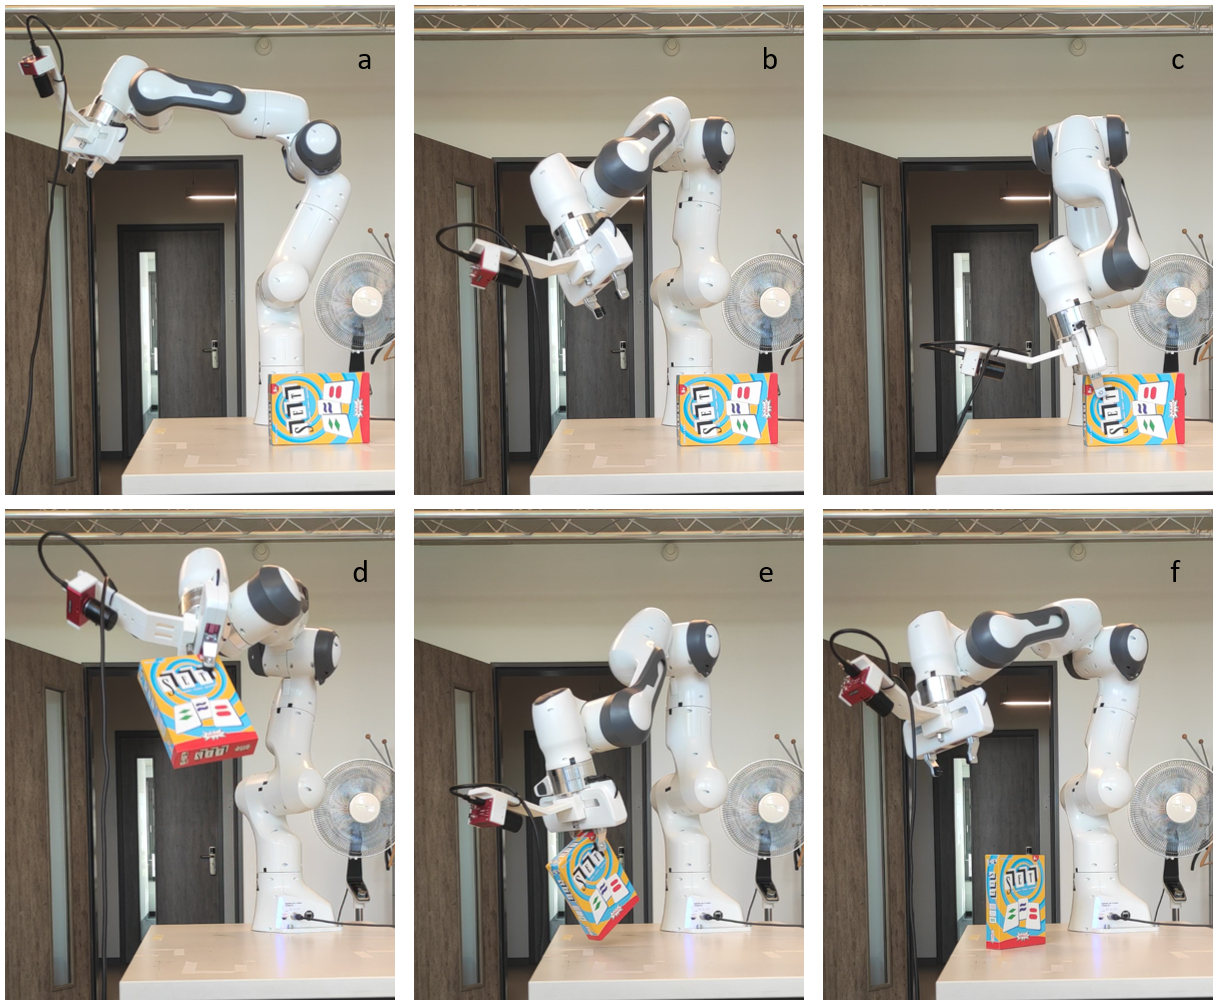
\includegraphics[width=\textwidth]{resources/images/rob_traj}
    \caption{Sequence of images (\textit{a-f}) showing an example pick-and-place motion.}\label{fig:rob_traj}
\end{figure}

During the experiments, a non-controlled background was present and textured objects were used in order to make sure events are generated if a slip occurs. This condition is not so strict, as most of the daily use objects have enough texture.\\

The first experiments were conducted with the goal of exploring different kinds of slip and grasp failures, with diverse objects. Then, we focused our efforts on a concrete type of slip and recorded more data. Furthermore, we recorded additional data in different scenarios including more sources of information into the dataset, which were required to explore other methods for slip detection.

\section{Initial data}

First, we had to think about how to generate slip or grasping failures during a pick-and-place motion. For that, in the literature, either the gripper's force is modified ~\cite{gelsight2017}, so that if it is not enough it will induce slip or grasp failure, or the gripper's width is modified ~\cite{gelsight2018}, so that if it is too wide the object will not be picked properly. However, we realized that the two-fingered gripper designed for Panda, that we are using, has a minimum force of 20 N, which is already enough to grasp and move lightweight objects and even heavy objects grasped from the center. Moreover, the gripper width has a binary behavior, either it closes until the indicated gripping force is reached, or it does not even close. Therefore, the only option to generate slip experiments by changing the gripper's force and/or width is by changing the gripper itself, for example, the Robotiq 2F-85 or 2F-140 would be suitable. Nevertheless, the acquisition of such gripper and redesign of the camera mount would require a significant amount of time, which is out of the time frame of this thesis.\\

So, some other options to induce slip or grasping failures have been found, as described in the following subsections.

\subsection{Off-centered grasping}

In ~\cite{rss2020} slip is generated by grasping the object away from its center of mass, which will induce some rotation in the object during the lifting phase, as happened in the sequence shown in ~\Cref{fig:rob_traj}.\\

A first slip sequence is shown in ~\Cref{fig:init_exp1}, where a heavy book is grasped from the corner, away from its center of mass. In the first event image, we can observe the edges of the two fingers of the grippers, as it is closing. Also some edges of the object are visible due to some movement provoked by the gripper. In the following two frames, events appear in the background, as the arm with the attached camera are moving, and from the object, due to rotational slip. It is worth noticing that there are no events coming from the end-effector and part of the camera mount, as they move rigidly with the camera, hence there is no difference in the pixels during the whole motion. Finally, once the slip stops, there are no more events coming from the book, which starts also moving rigidly with respect to the camera, as happens in the last frame.

\begin{figure}[h]
    \centering
    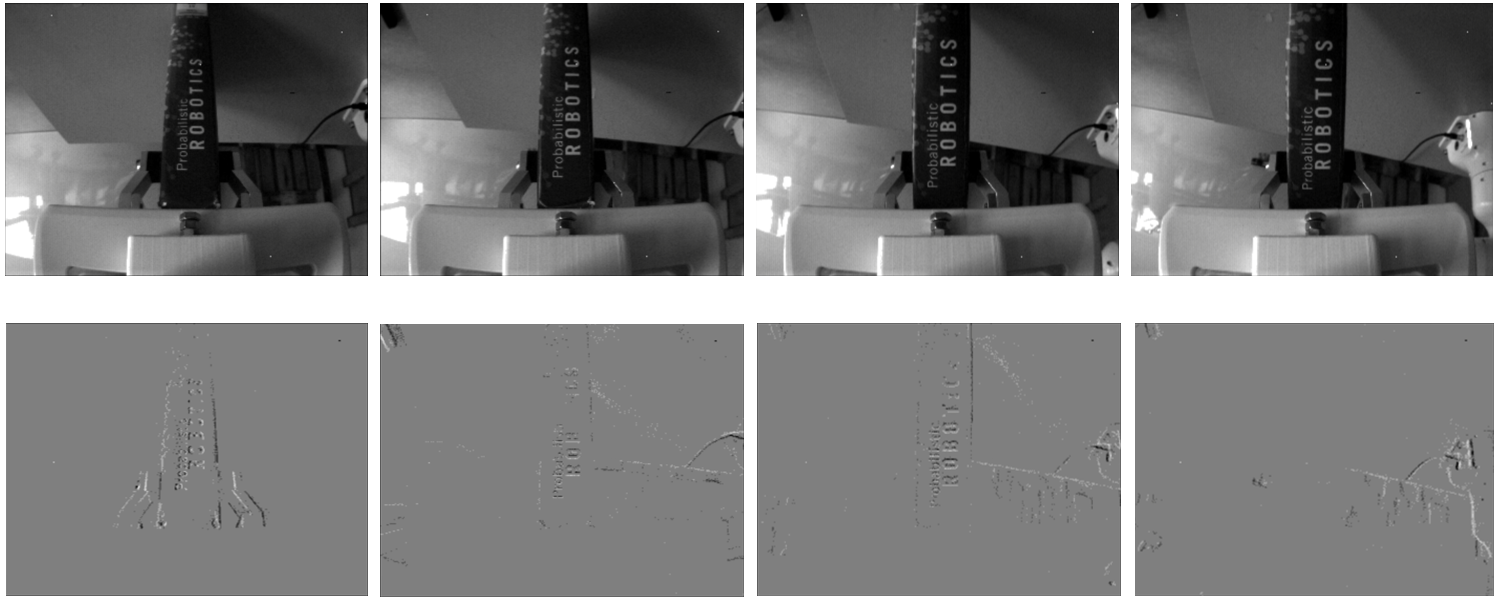
\includegraphics[width=\textwidth]{resources/images/init_exp1}
    \caption{Sequence of grayscale frames (first row) and event images (second row) during a slip, while executing a pick-and-place motion with a book.}\label{fig:init_exp1}
\end{figure}

Another sequence of off-centered grasping is depicted in ~\Cref{fig:init_exp2}, where a hammer is grasped from the bottom of its handle, having the center of mass quite far from the gripper, because of the weight of its head. Due to the high momentum generated while lifting the hammer, the object starts to swing fastly and it slips away from the gripper, provoking a grasping failure, as observed in the last frame. Again the event images are really informative of this failure, as events come and form a map of moving edges indicating the relative movement of the hammer with respect to the camera. As expected, there are also events coming from the background and, in the last frame, events come also from the two fingers of the gripper, because they close when the object slips through the fingers.

\begin{figure}[H]
    \centering
    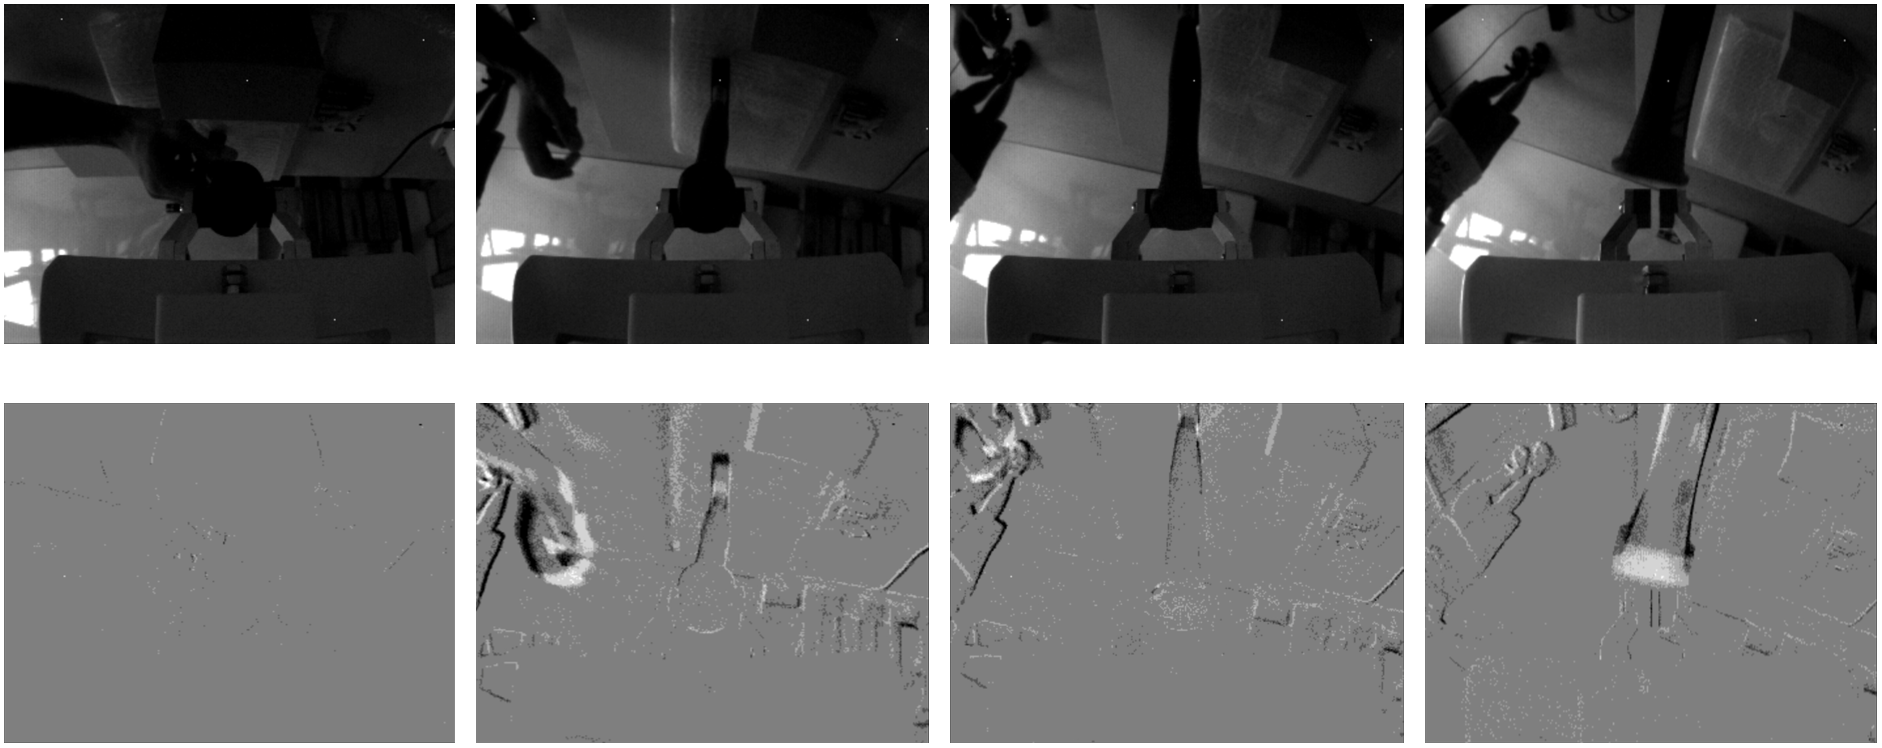
\includegraphics[width=\textwidth]{resources/images/init_exp2}
    \caption{Sequence of grayscale frames (first row) and event images (second row) during a grasp failure, while executing a pick-and-place motion with a hammer.}\label{fig:init_exp2}
\end{figure}

\subsection{Pulling with string}

An alternative way of forcing rotational slip, is by attaching a string to the object and pulling it, applying force to the object and forcing it to rotate. This might seem a synthetic scenario, but actually it resembles a real case where an object is picked in a cluttered environment and maybe the grasped object is attached to another object and gets pulled by it.\\

An example sequence is represented in ~\Cref{fig:init_exp3}, where first the object is pulled upwards (downwards in the images as they are inverted), generating the moving edges in the second event image. Then the object is pulled downwards (upwards in the images), with a clearly visible movement in the third event image. Finally, there are no more slips and no more events appear from the object in the fourth event image.

\begin{figure}[H]
    \centering
    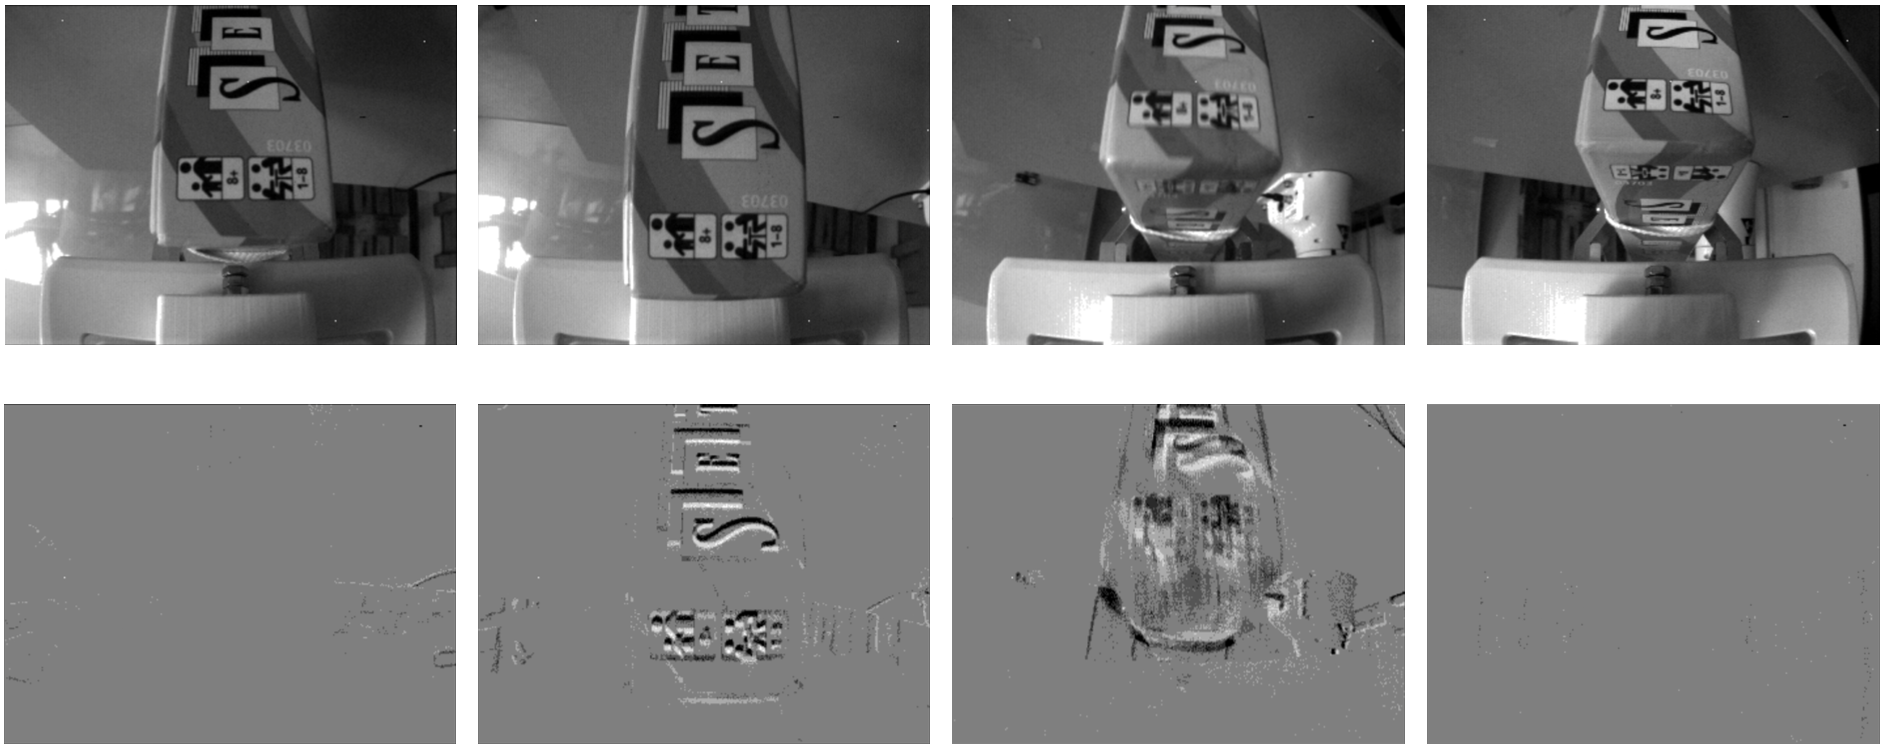
\includegraphics[width=\textwidth]{resources/images/init_exp3}
    \caption{Sequence of grayscale frames (first row) and event images (second row) during two slips generated by an external force, while executing a pick-and-place motion with a box.}\label{fig:init_exp3}
\end{figure}

\subsection{Deformable objects}

Until now only rigid bodies have been considered, however, instead of grasping the book as in ~\Cref{fig:init_exp1}, we can grasp some of its pages and the object will behave as a non-rigid body. In ~\Cref{fig:init_exp4} an example sequence is shown with this scenario, where we can observe how the book opens after lifting it and the non-grasped part of the book swings during the whole motion, which is visible through the edges of the book in the event images. Nevertheless, this is not a slip nor a grasping failure, it is a continuous swinging of part of the object, which may be useful to detect as it may damage it.

\begin{figure}[H]
    \centering
    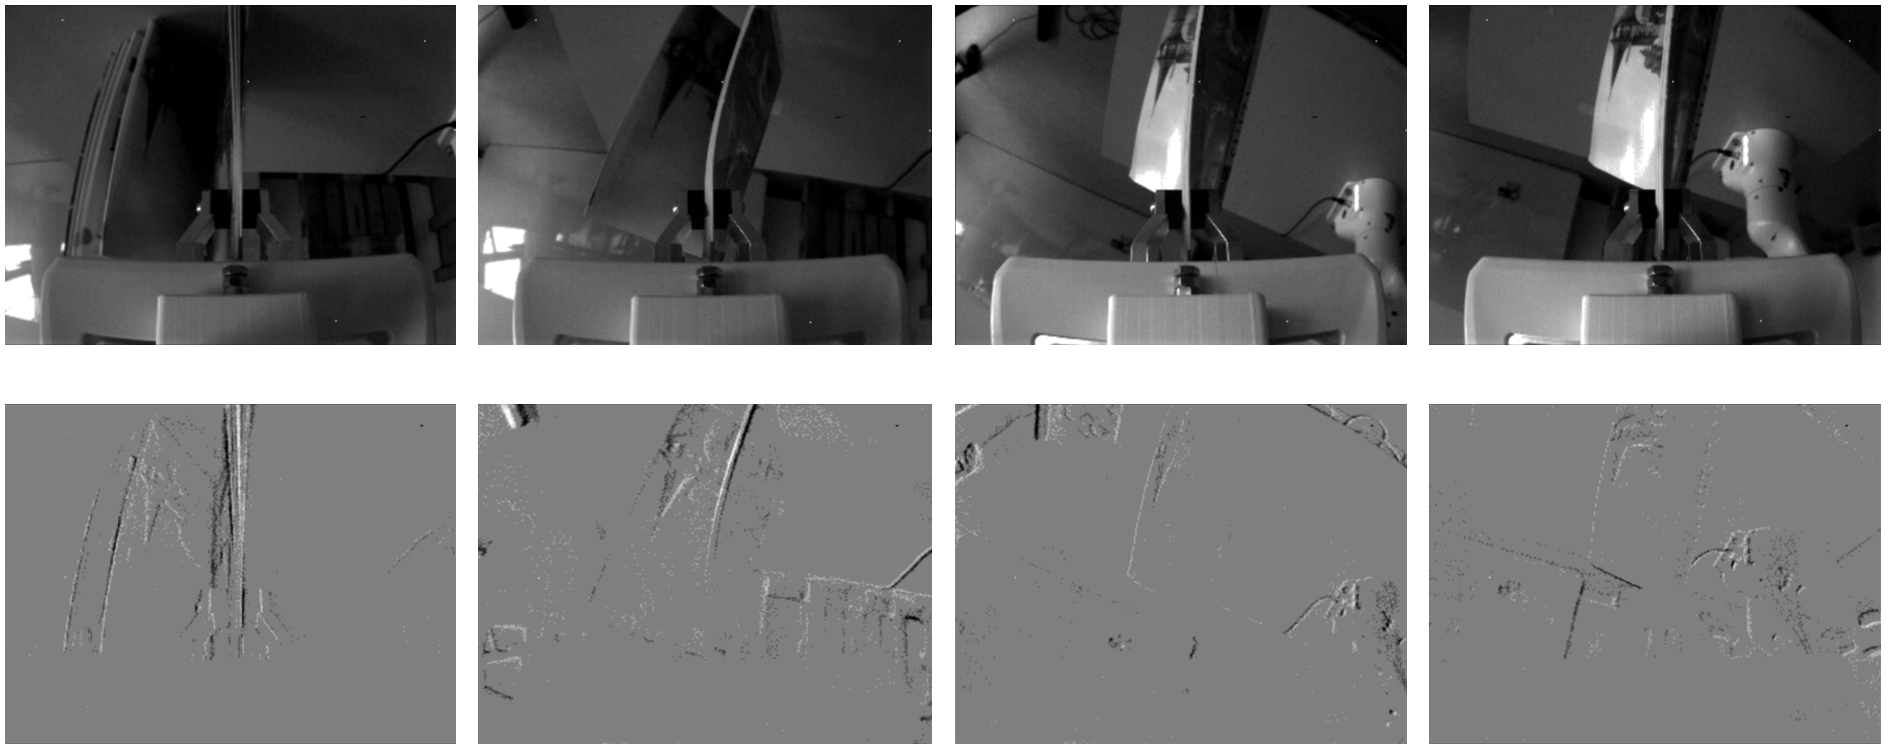
\includegraphics[width=\textwidth]{resources/images/init_exp4}
    \caption{Sequence of grayscale frames (first row) and event images (second row) during swinging, while executing a pick-and-place motion with an open book.}\label{fig:init_exp4}
\end{figure}

\section{Set 1}

After analyzing different ways of generating slip and grasping failures, we focused our efforts in studying in deep off-centered grasping using rigid bodies. This kind of grasping generates rotational slip in the beginning, which can be detected and the object can be placed again in the initial position and re-grasped from another point to make sure the pick-and-place motion occurs without slippage.\\

In ~\Cref{fig:set1_case1} a first example sequence can be observed, with a box which has a heavy mass inside in the other side of the grasping point, in order to induce slip. However, in this case there is only a slight rotation of the object, which can be appreciated thanks to the edges of the second event image.

\begin{figure}[H]
    \centering
    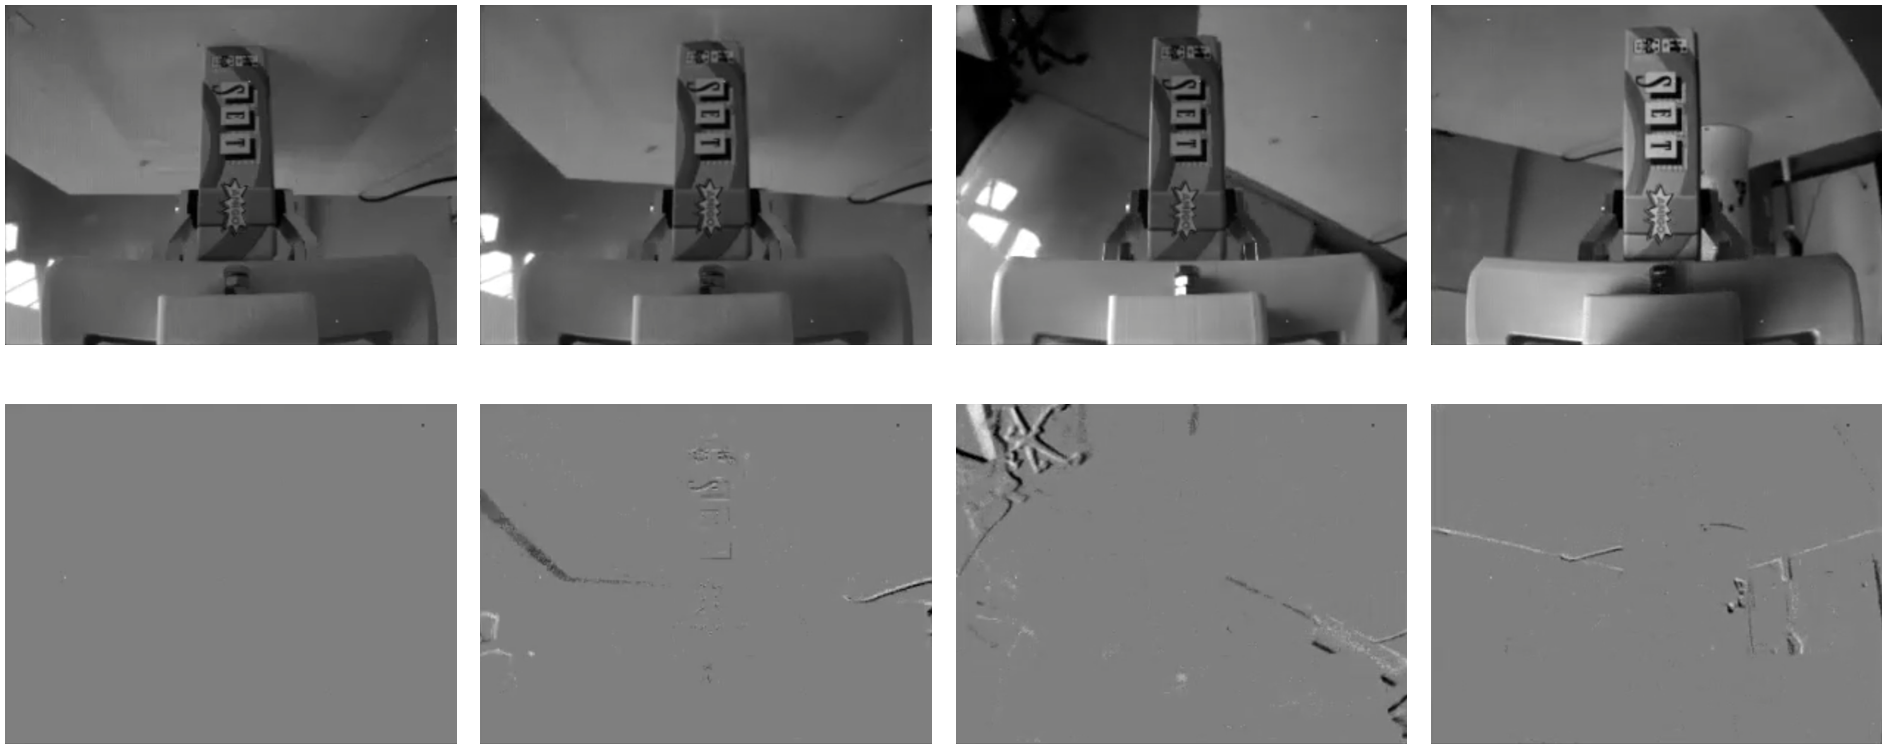
\includegraphics[width=\textwidth]{resources/images/set1_case1}
    \caption{Sequence of grayscale frames (first row) and event images (second row) during a minor slip, while executing a pick-and-place motion with a box.}\label{fig:set1_case1}
\end{figure}

On the contrary, in ~\Cref{fig:set1_case2}, a significant slip occurs in the same scenario, varying slightly the grasping point. First, the object rotates in one direction, as observed in the second frame, and then it rotates in the opposite direction, which can be appreciated in the third frame. To see the direction of rotation by looking at the event images, we can focus on the letter \textit{S}, which is black over a white background. If the \textit{S} moves downwards, as happens in the second frame, the pixels below will change their value from white (high value in grayscale) to the black pixels (low value in grayscale) of the letter \textit{S}, generating events with negative polarity (represented with black shades in the event image). Oppositely, the pixels in the \textit{S} change from black to white, generating events with positive polarity (represented with white shades in the event image). In contrast, in the third frame the event polarities are switched with respect to the previous frame, therefore, the \textit{S} is moving upwards, indicating a change in the direction of slip. Finally, the slip ends and the place motion is completed without additional slips, as there are no moving edges in the last frame.

\begin{figure}[H]
    \centering
    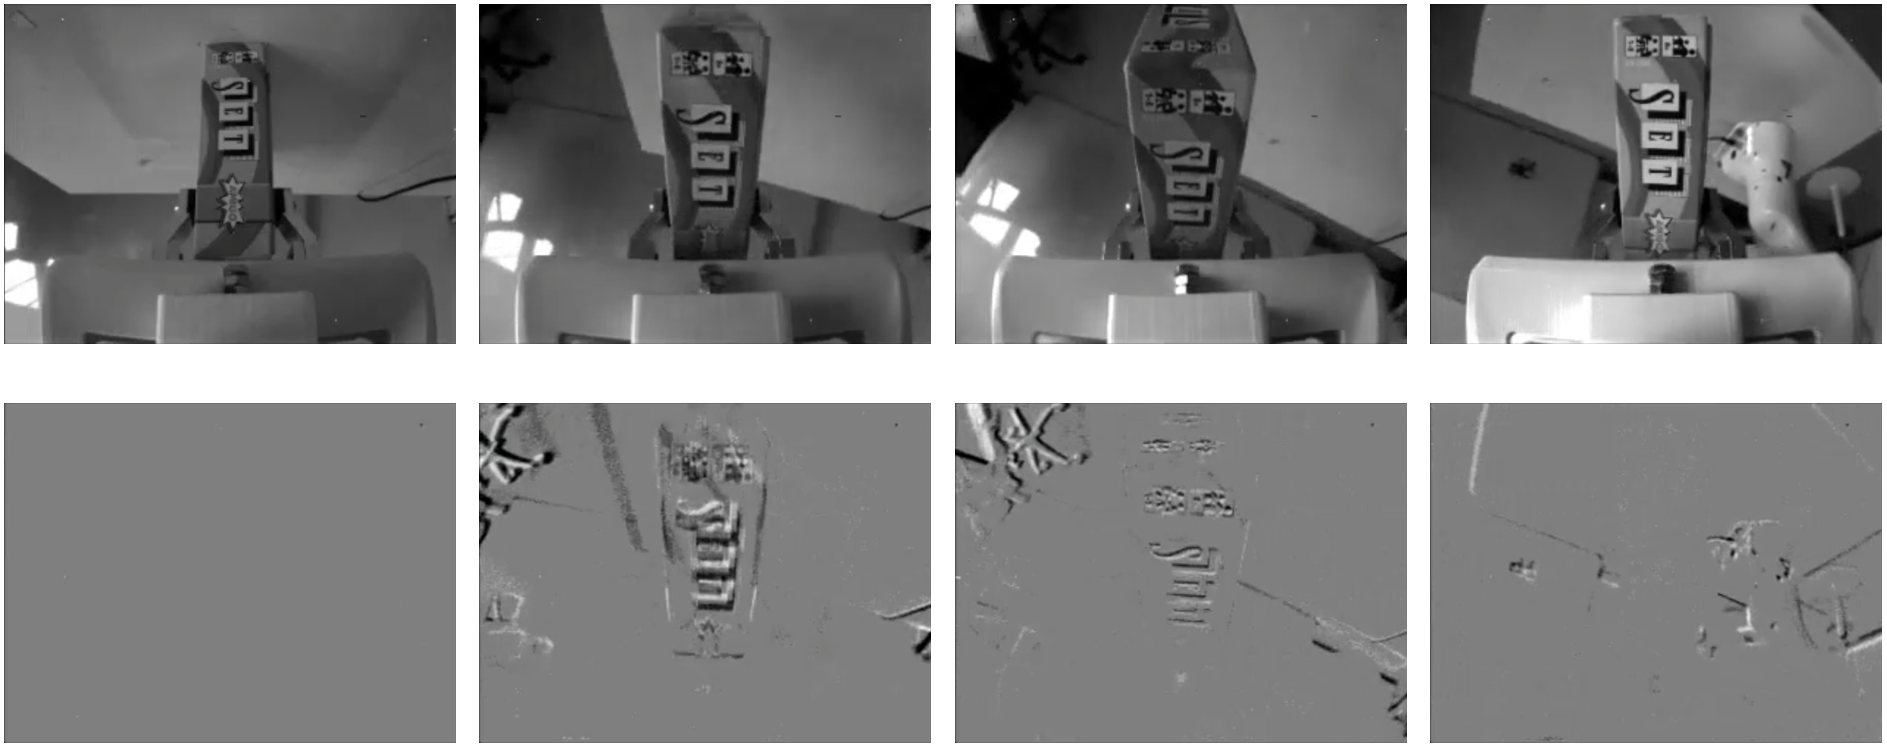
\includegraphics[width=\textwidth]{resources/images/set1_case2}
    \caption{Sequence of grayscale frames (first row) and event images (second row) during a significant slip, while executing a pick-and-place motion with a box.}\label{fig:set1_case2}
\end{figure}

Changing the object, and using instead a book, we can observe a similar behavior, as depicted in ~\Cref{fig:set1_case3}. In the second frame a slip is visible, thanks to the moving edges shown in the event image, which are generated by the letters on the book's cover. Then, in the third frame, the slip seems to stop, but the rotation continues to the other direction, as shown in the fourth frame. It is worth noticing that, if there were no letters on the cover, meaning no texture in the object, there would not be any events caused by the slips.\\

\begin{figure}[h]
    \centering
    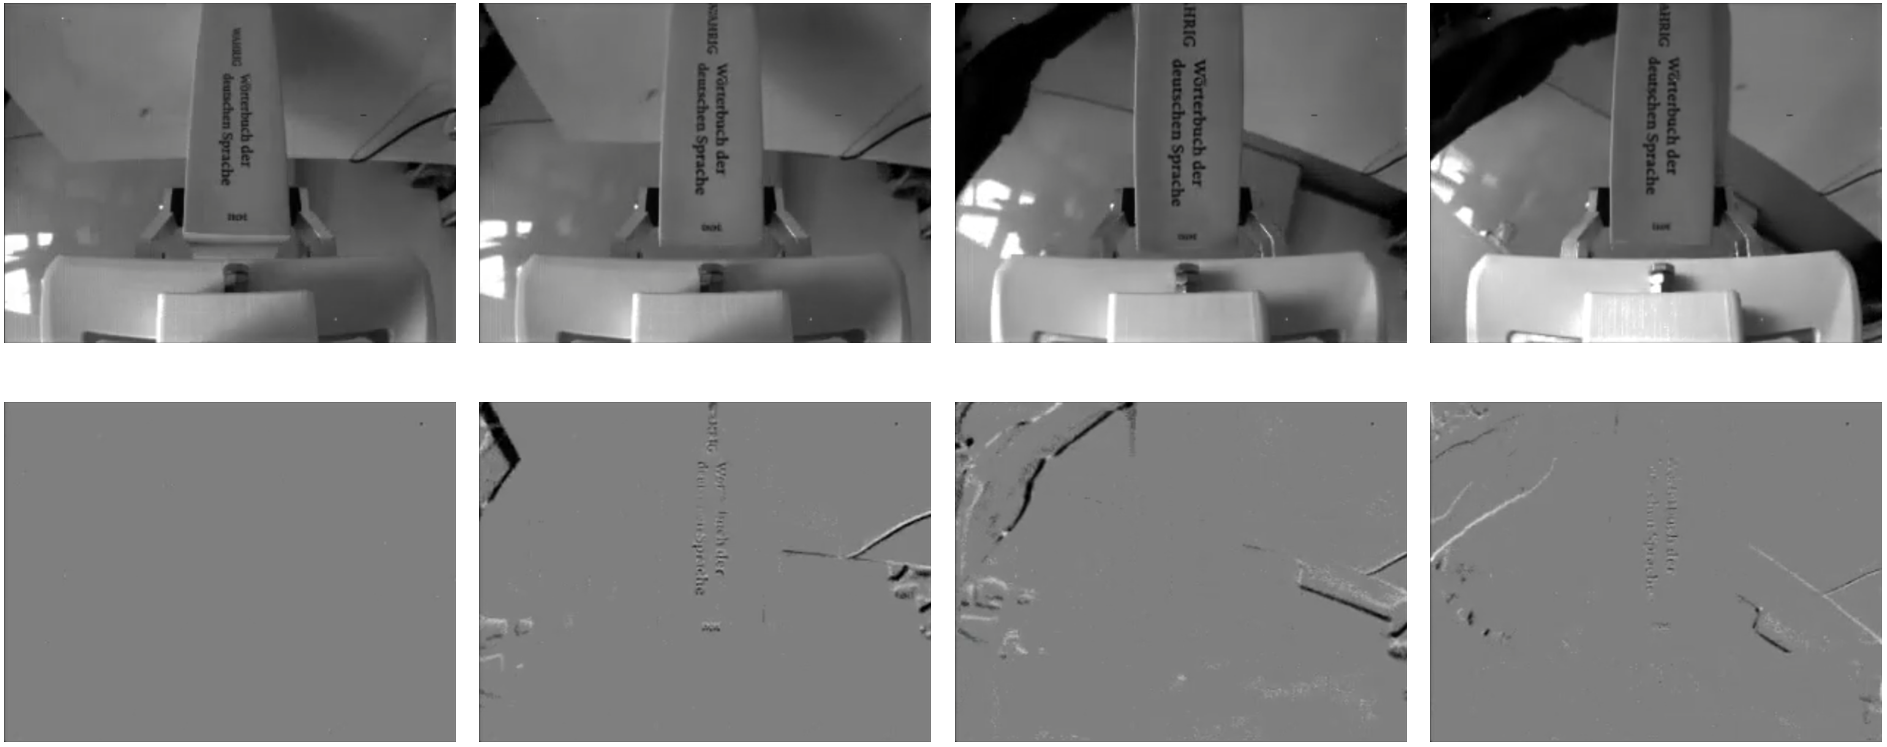
\includegraphics[width=\textwidth]{resources/images/set1_case3}
    \caption{Sequence of grayscale frames (first row) and event images (second row) during a significant slip, while executing a pick-and-place motion with book no. 1.}\label{fig:set1_case3}
\end{figure}

Using another book, with more texture, see ~\Cref{fig:set1_case4}, only one slip occurs in the second frame. Thanks to having more texture, the edges in the event image are more visible.\\

\begin{figure}[h]
    \centering
    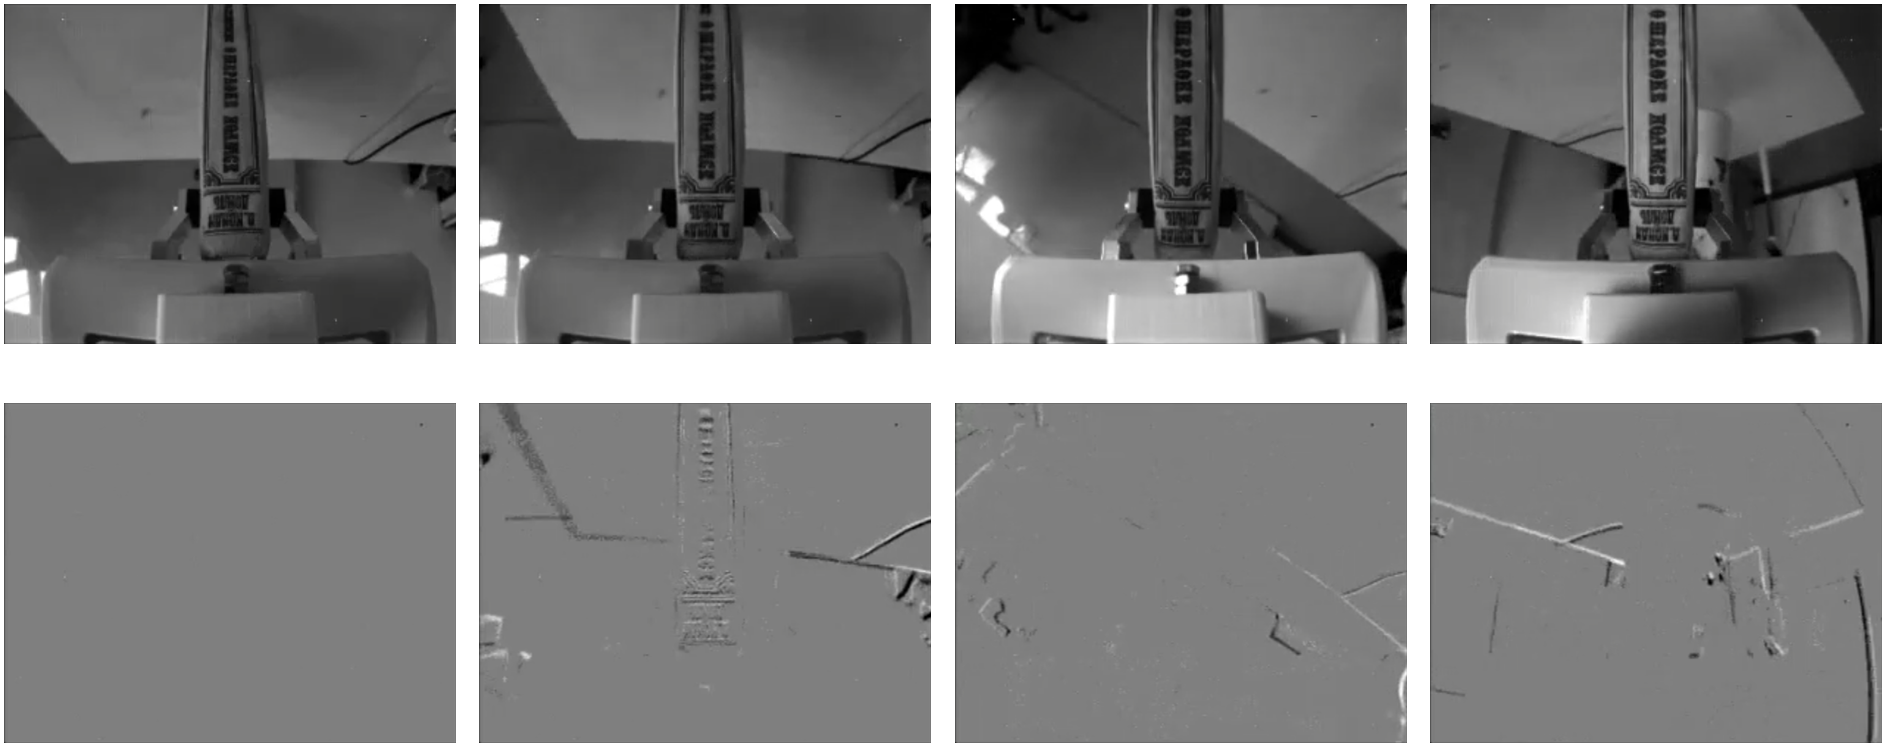
\includegraphics[width=\textwidth]{resources/images/set1_case4}
    \caption{Sequence of grayscale frames (first row) and event images (second row) during a significant slip, while executing a pick-and-place motion with book no. 2.}\label{fig:set1_case4}
\end{figure}

The same book, can be grasped just from the opposite side of it, so that the rotational slip occurs in the other direction. In ~\Cref{fig:set1_case5}, we can see the slip happening in the second and third frames. This experiment is relevant also to see the effects of having the object really close to the camera in the beginning of the motion.\\

\begin{figure}[h]
    \centering
    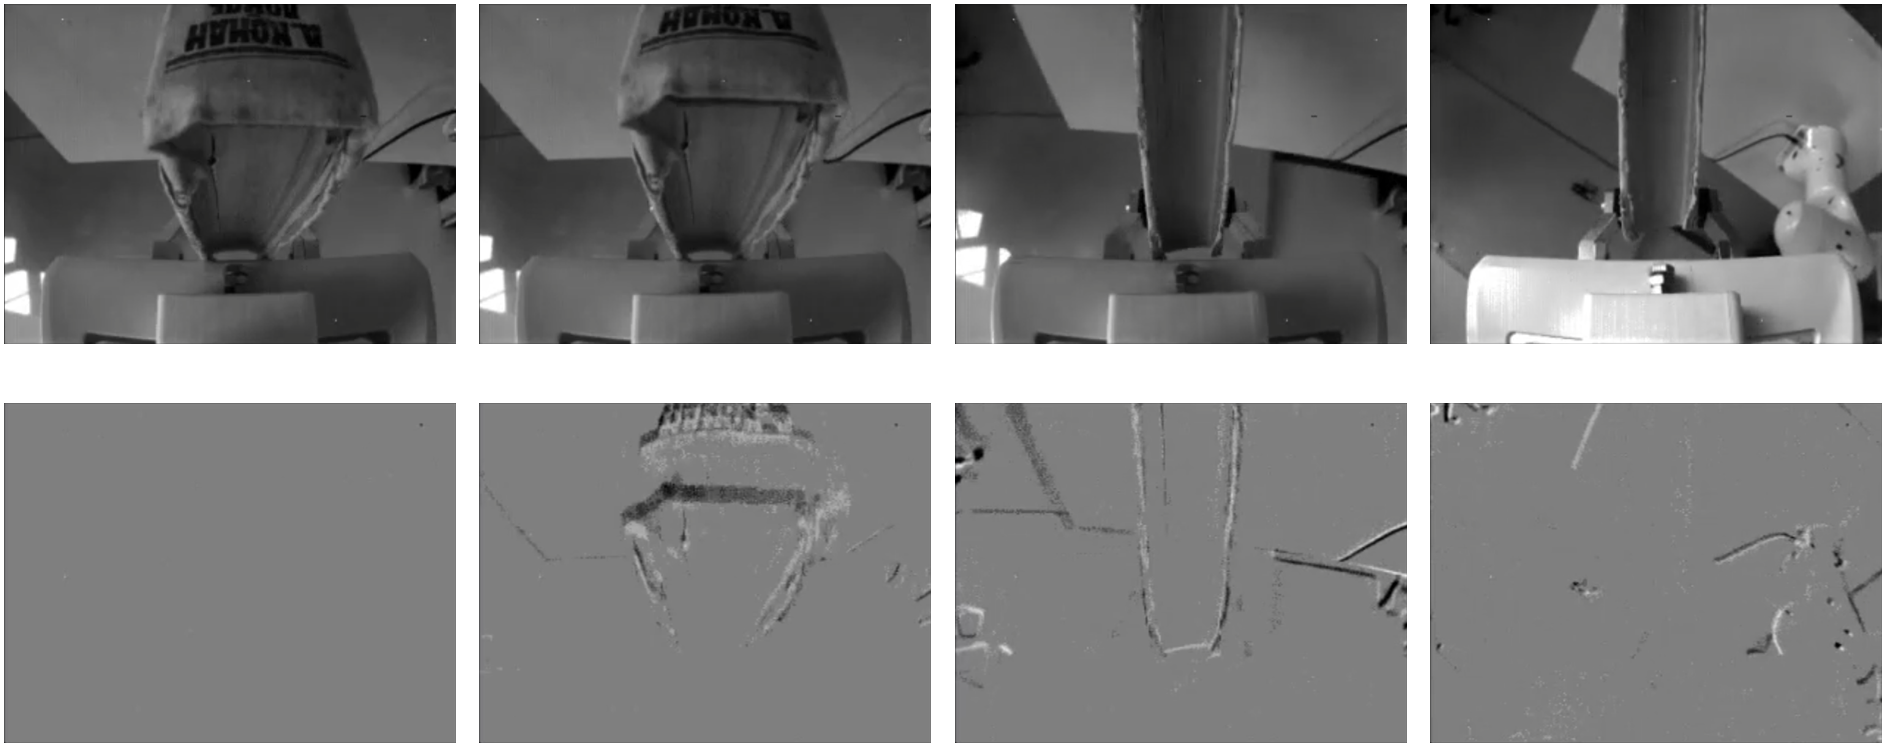
\includegraphics[width=\textwidth]{resources/images/set1_case5}
    \caption{Sequence of grayscale frames (first row) and event images (second row) during a significant slip, while executing a pick-and-place motion with book no. 2 and reverse grip.}\label{fig:set1_case5}
\end{figure}

This same scenario can be replicated with the box used in the first experiments, as shown in ~\Cref{fig:set1_case6}. The slip is similar to the previous case, but now more events appear, thanks to the highly textured object, and the box is even closer to the camera.

\clearpage

\begin{figure}[h]
    \centering
    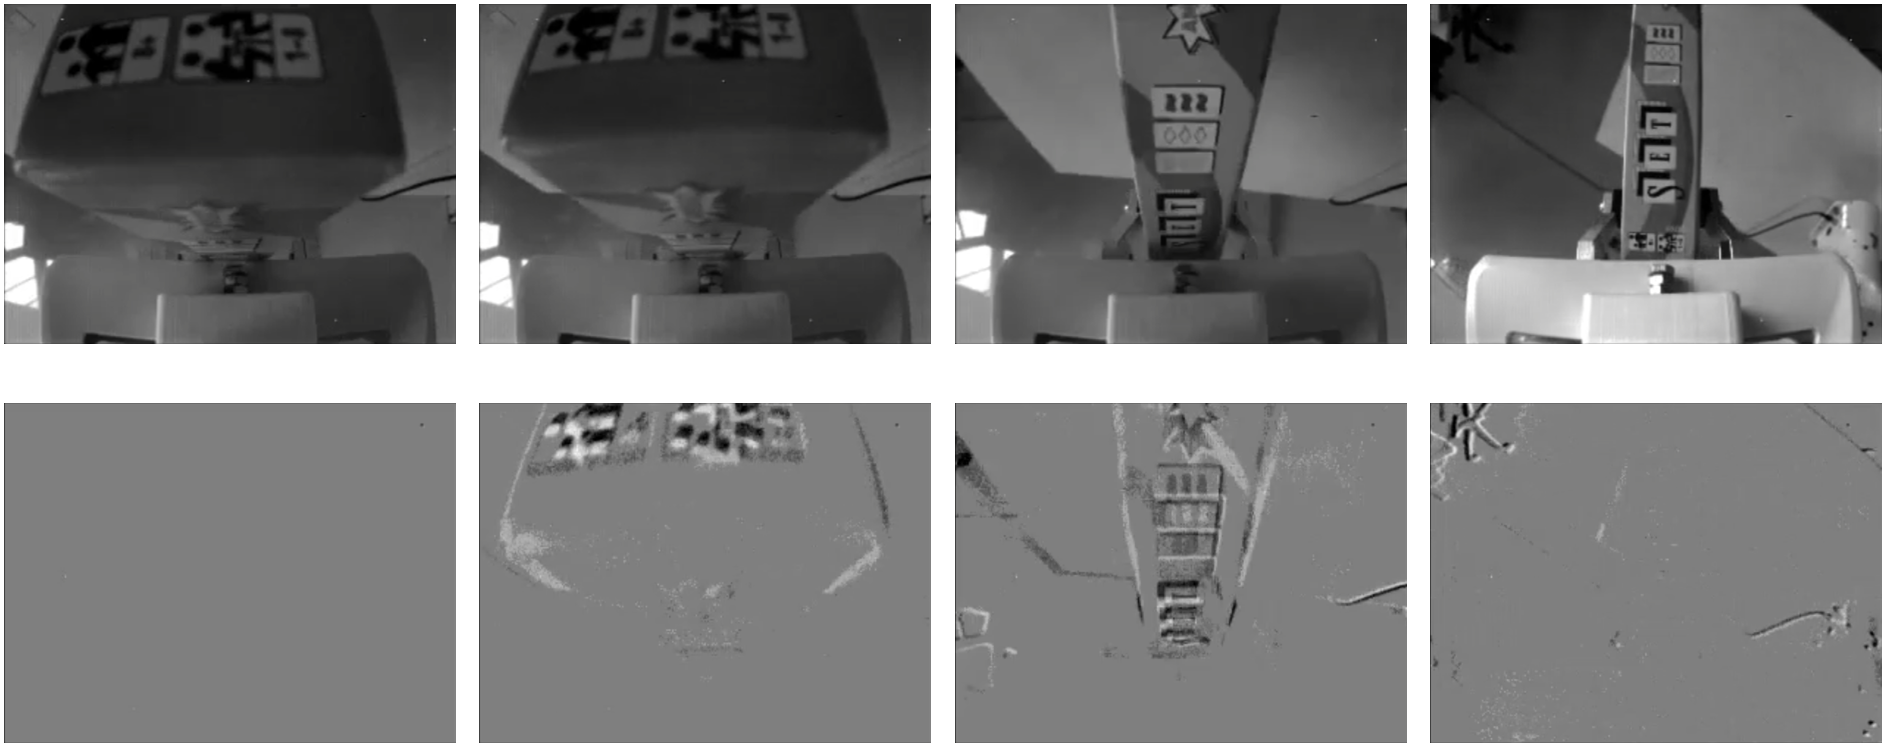
\includegraphics[width=\textwidth]{resources/images/set1_case6}
    \caption{Sequence of grayscale frames (first row) and event images (second row) during a significant slip, while executing a pick-and-place motion with a box and reverse grip.}\label{fig:set1_case6}
\end{figure}

Finally, the book used in ~\Cref{fig:set1_case3} is used again but changing the texture of the background. Concretely, a mat of photos has been placed on the table. In ~\Cref{fig:set1_case7}, the resulting sequence is shown, where the events coming from the book are similar compared to ~\Cref{fig:set1_case3}, but the background has many more moving edges in the event images. It is quite important to try also different background scenarios, to make sure that the developed methods do generalize in such conditions, or at least to know their limitations.

\begin{figure}[H]
    \centering
    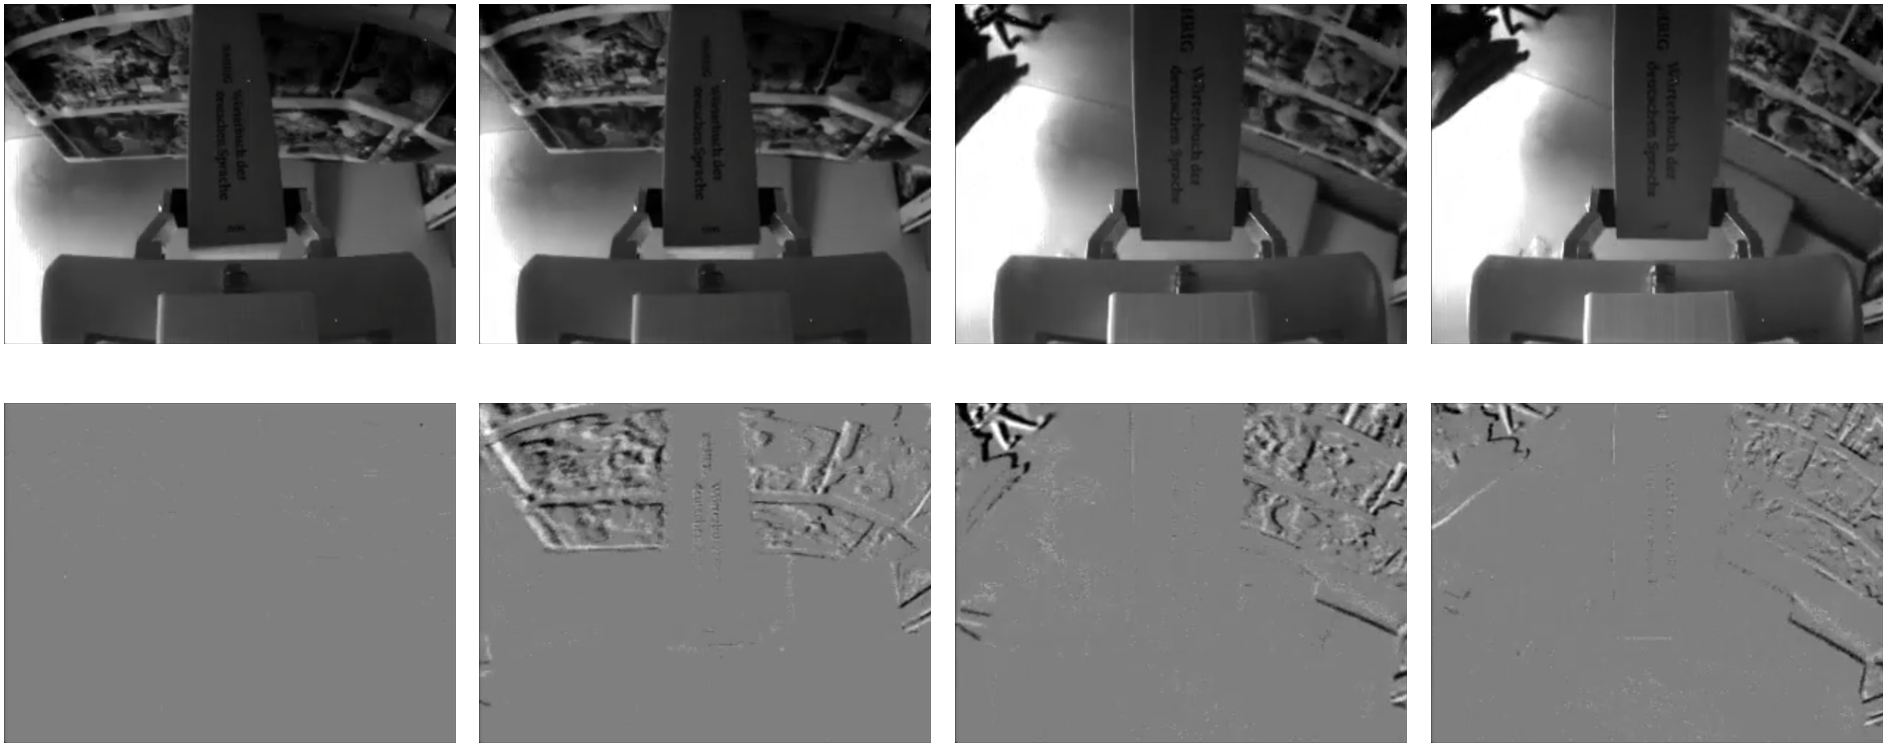
\includegraphics[width=\textwidth]{resources/images/set1_case7}
    \caption{Sequence of grayscale frames (first row) and event images (second row) during a significant slip, while executing a pick-and-place motion with book no. 1 and a highly textured table.}\label{fig:set1_case7}
\end{figure}

It is worth mentioning that all these experiments have been repeated 4-6 times in order to check the repeatability during the analysis of the slip detection.

\section{Set 2}

While analyzing Set 1, we realized that including the camera angular velocity would be informative to compute the motion flow in the scene and recording a sequence without grasping any object would enable us to compare against a sequence with an object and identify where the object located in the scene. These are the reasons behind recording a new set of data.\\

Moreover, in Set 1, the recorded data were mostly slip cases, so for this new set a balanced amount of slip and non-slip sequences has been recorded (3-5 times for each scenario).\\

In ~\Cref{fig:set2_empty} the usual trajectory is executed without grasping any object. Then, as shown in ~\Cref{fig:set2_case1}, a book is picked and no slip occurs during the whole sequence, which is accomplished by grasping the book approximately from its center and using a higher gripping force. In contrast, in ~\Cref{fig:set2_case2}, by grasping from the edge and using a lower force, a slip can be observed. Moreover, grasping from the other end of the book, there is a slip in the opposite direction, as depicted in ~\Cref{fig:set2_case3}.\\

Similarly, using another book, a non-slip case is observed in ~\Cref{fig:set2_case4} and a slip case is represented in ~\Cref{fig:set2_case5}.

\begin{figure}[H]
    \centering
    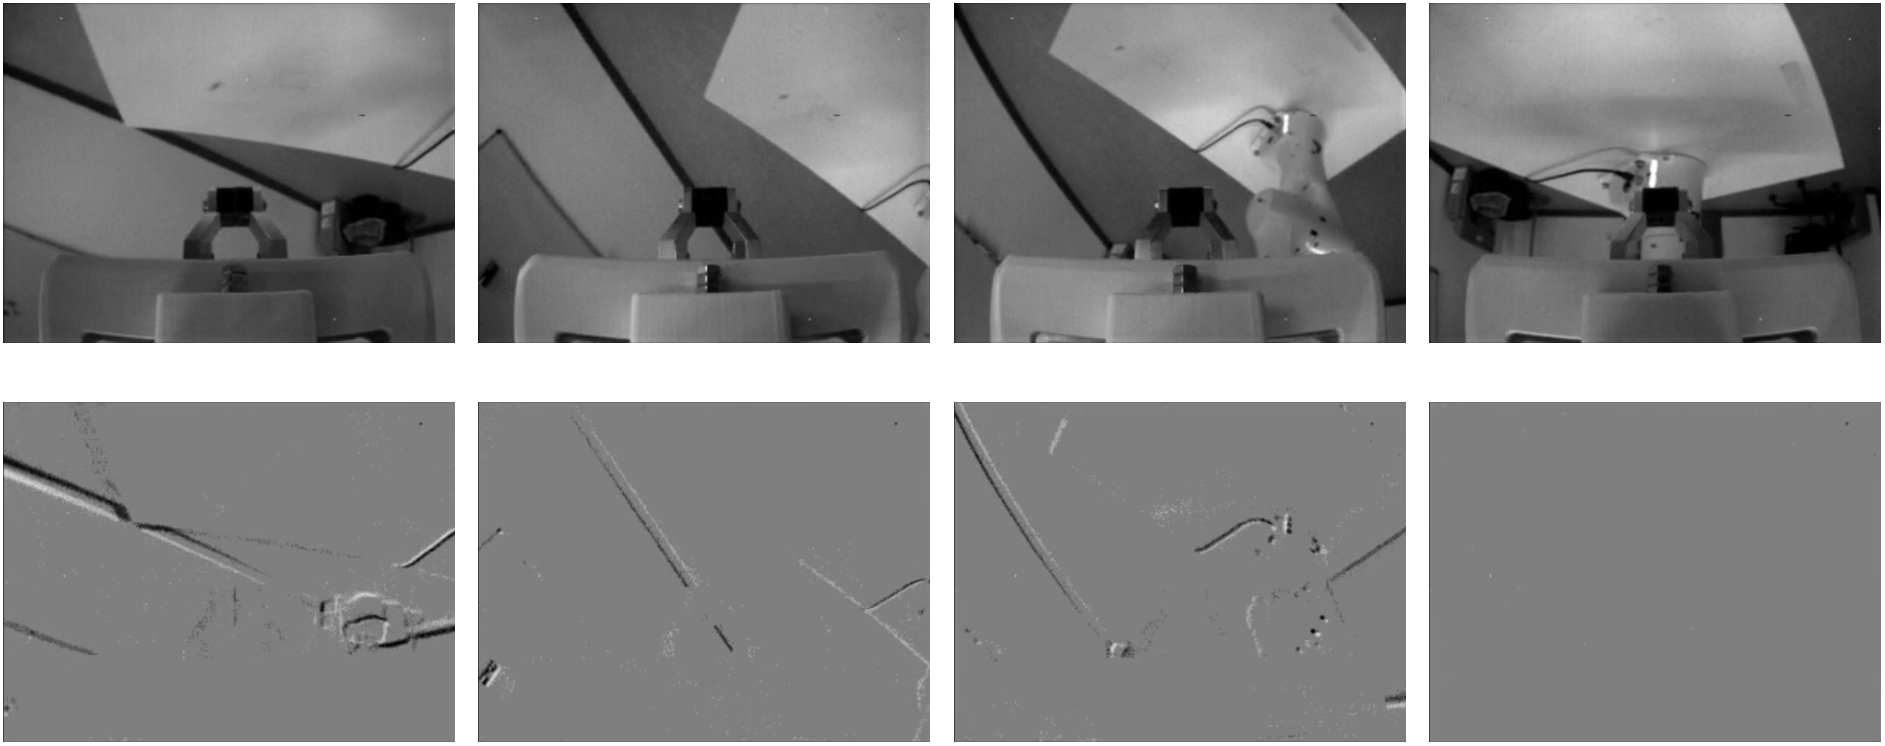
\includegraphics[width=\textwidth]{resources/images/set2_empty}
    \caption{Sequence of grayscale frames (first row) and event images (second row) while executing a pick-and-place motion without any object.}\label{fig:set2_empty}
\end{figure}

\begin{figure}[H]
    \centering
    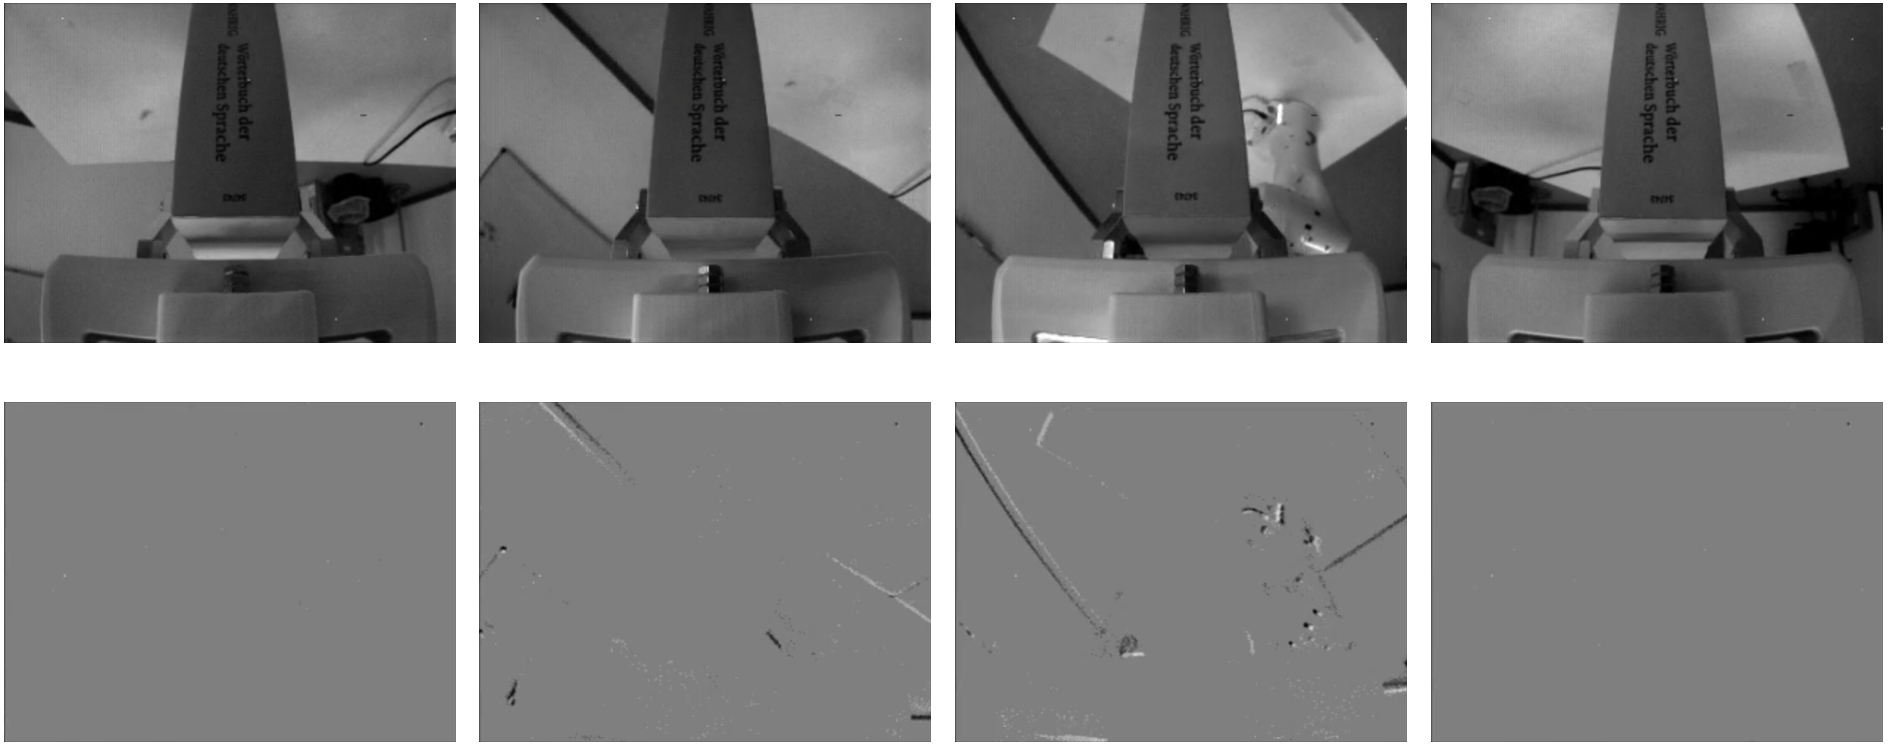
\includegraphics[width=\textwidth]{resources/images/set2_case1}
    \caption{Sequence of grayscale frames (first row) and event images (second row) during no slip, while executing a pick-and-place motion with book no. 1.}\label{fig:set2_case1}
\end{figure}

\begin{figure}[H]
    \centering
    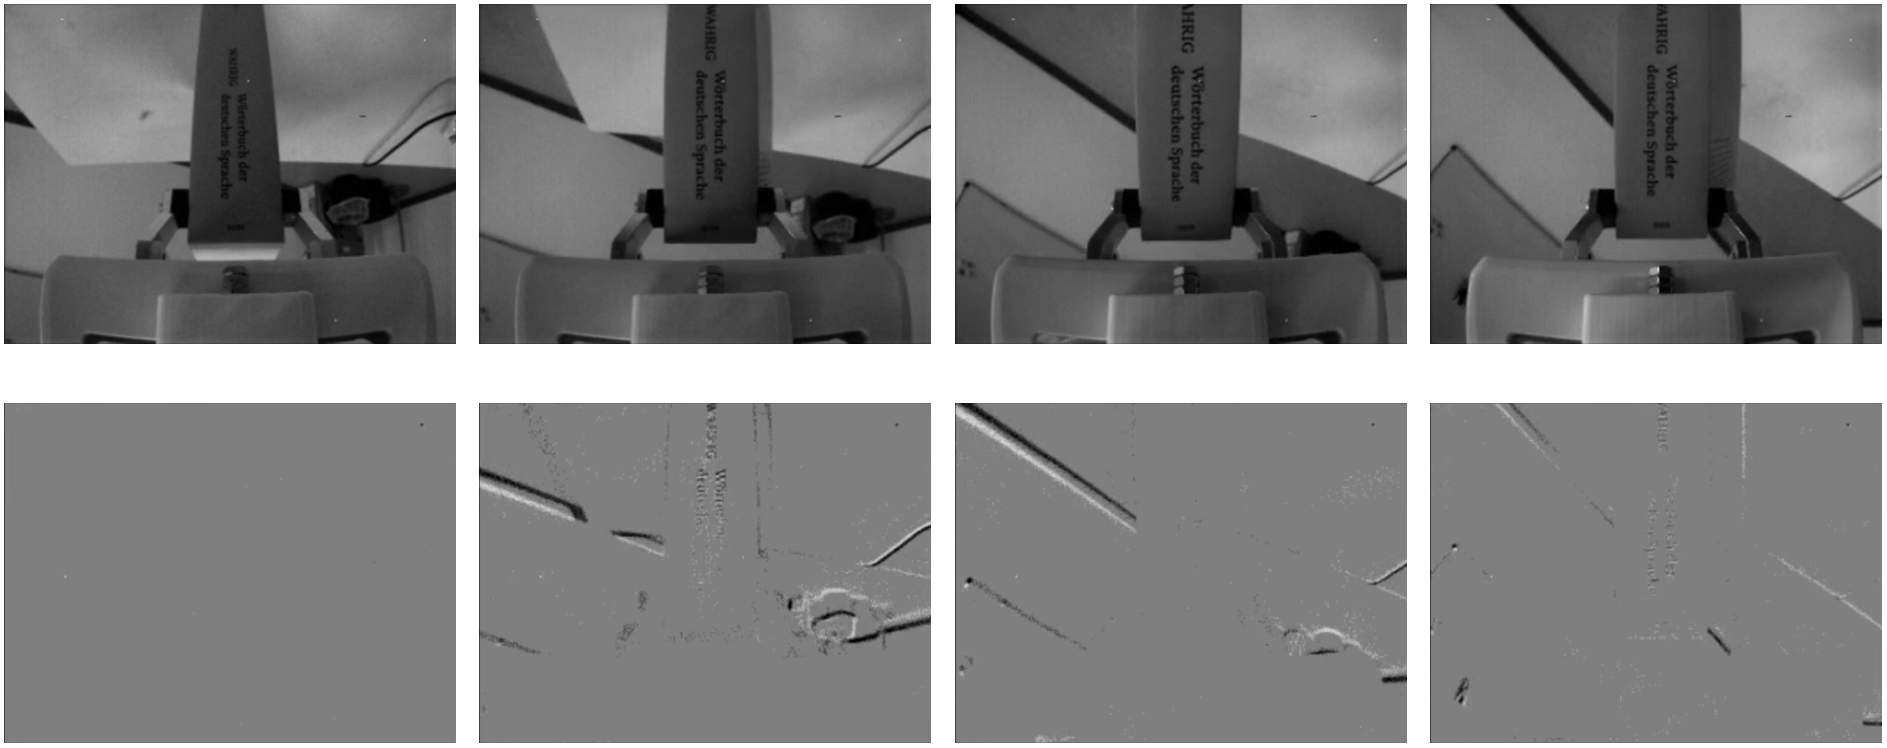
\includegraphics[width=\textwidth]{resources/images/set2_case2}
    \caption{Sequence of grayscale frames (first row) and event images (second row) during a significant slip, while executing a pick-and-place motion with book no. 1.}\label{fig:set2_case2}
\end{figure}

\begin{figure}[H]
    \centering
    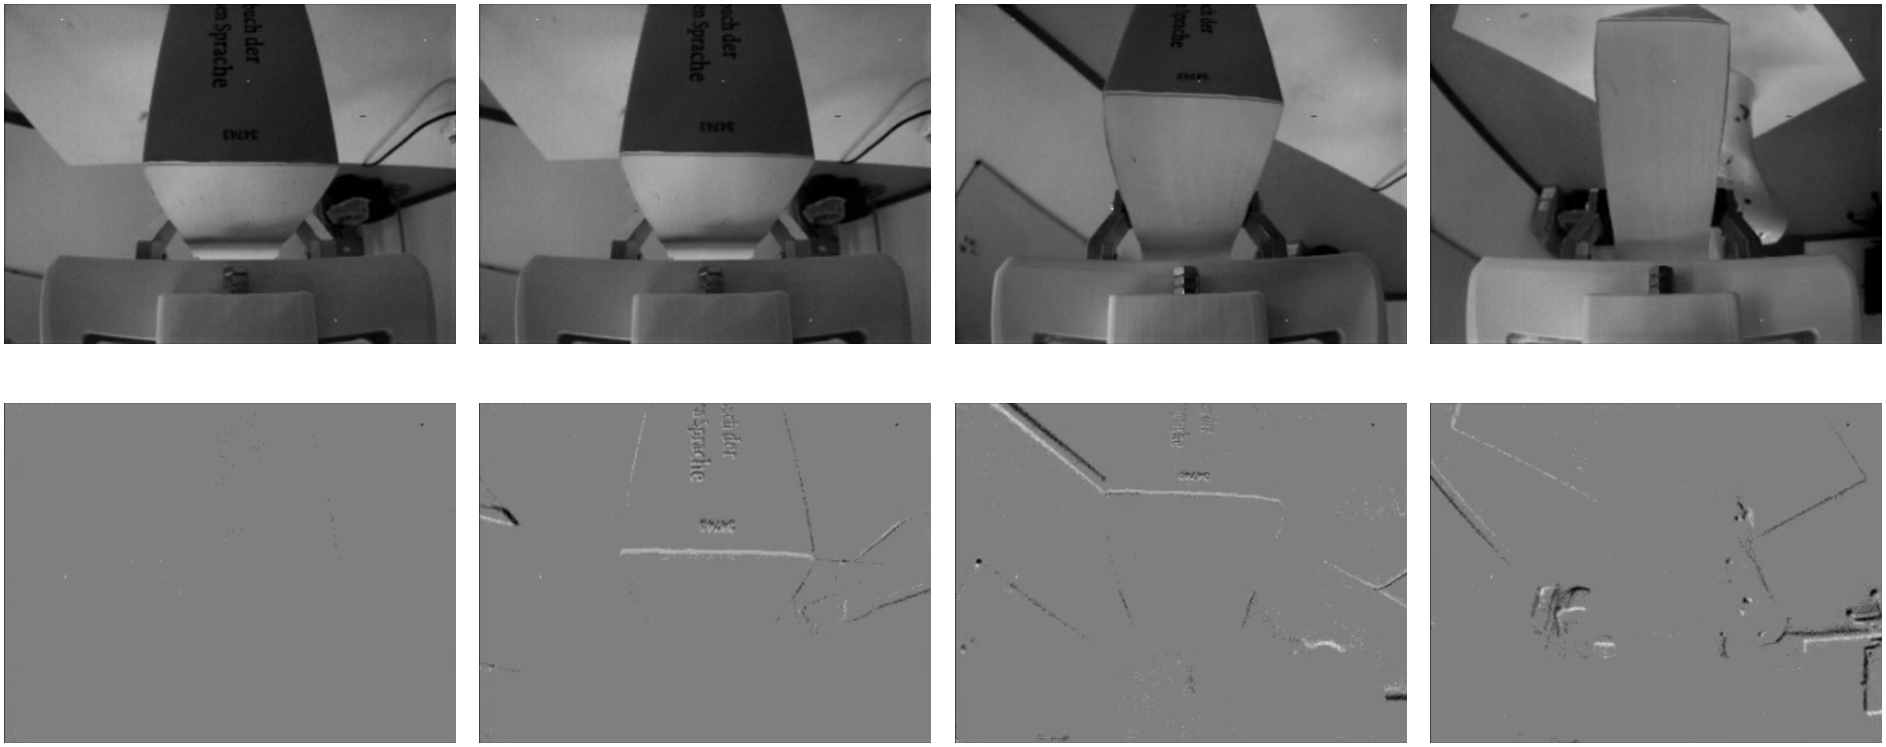
\includegraphics[width=\textwidth]{resources/images/set2_case3}
    \caption{Sequence of grayscale frames (first row) and event images (second row) during a significant slip, while executing a pick-and-place motion with book no. 1.}\label{fig:set2_case3}
\end{figure}

\begin{figure}[H]
    \centering
    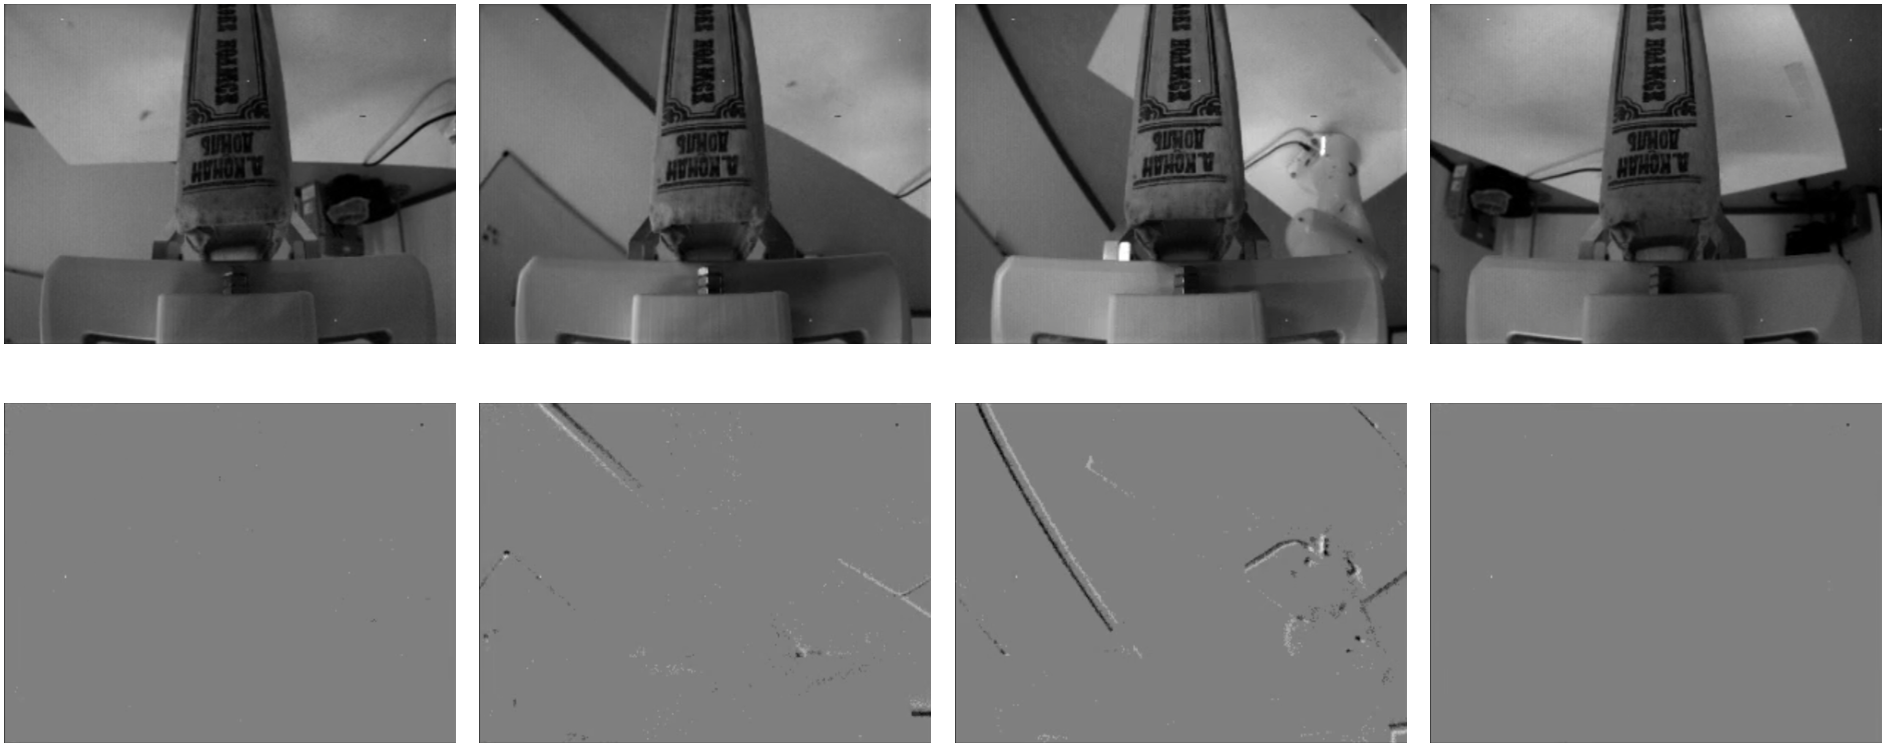
\includegraphics[width=\textwidth]{resources/images/set2_case4}
    \caption{Sequence of grayscale frames (first row) and event images (second row) during no slip, while executing a pick-and-place motion with book no. 2.}\label{fig:set2_case4}
\end{figure}

\begin{figure}[H]
    \centering
    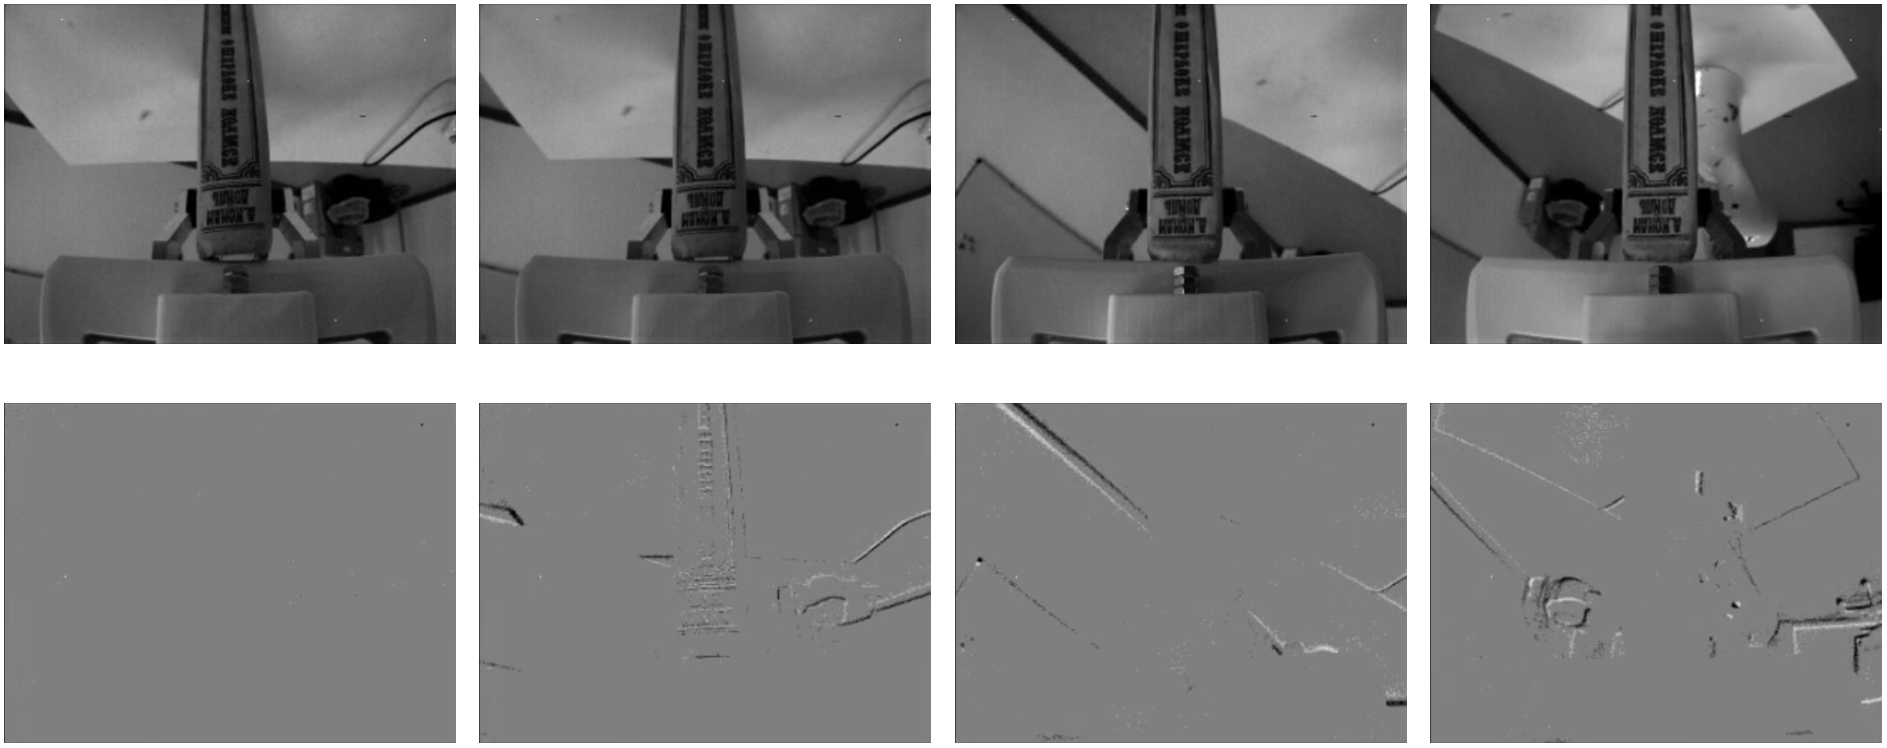
\includegraphics[width=\textwidth]{resources/images/set2_case5}
    \caption{Sequence of grayscale frames (first row) and event images (second row) during a significant slip, while executing a pick-and-place motion with book no. 2.}\label{fig:set2_case5}
\end{figure}

\section{Set 3}

The previous sets of data present one issue: the labeling of the time when a slip occurs has to be done manually. To solve this issue, ground-truth data should be saved in parallel with the rest of the data gathered until now. Concretely, we use a motion capture system, called OptiTrack, which consists of several cameras that track certain markers. These markers can be placed in rigid bodies and, once they are defined as so in \textit{Motive} (a optical motion capture software), the objects can be tracked with positional accuracies of $\pm 0.2$ mm and rotational accuracies of $\pm 0.1$º. In ~\Cref{fig:optitrack}, the new experiment setup is shown, with the OptiTrack cameras located at the top, and the object with markers shown in the bottom right part. 

\begin{figure}[H]
    \centering
    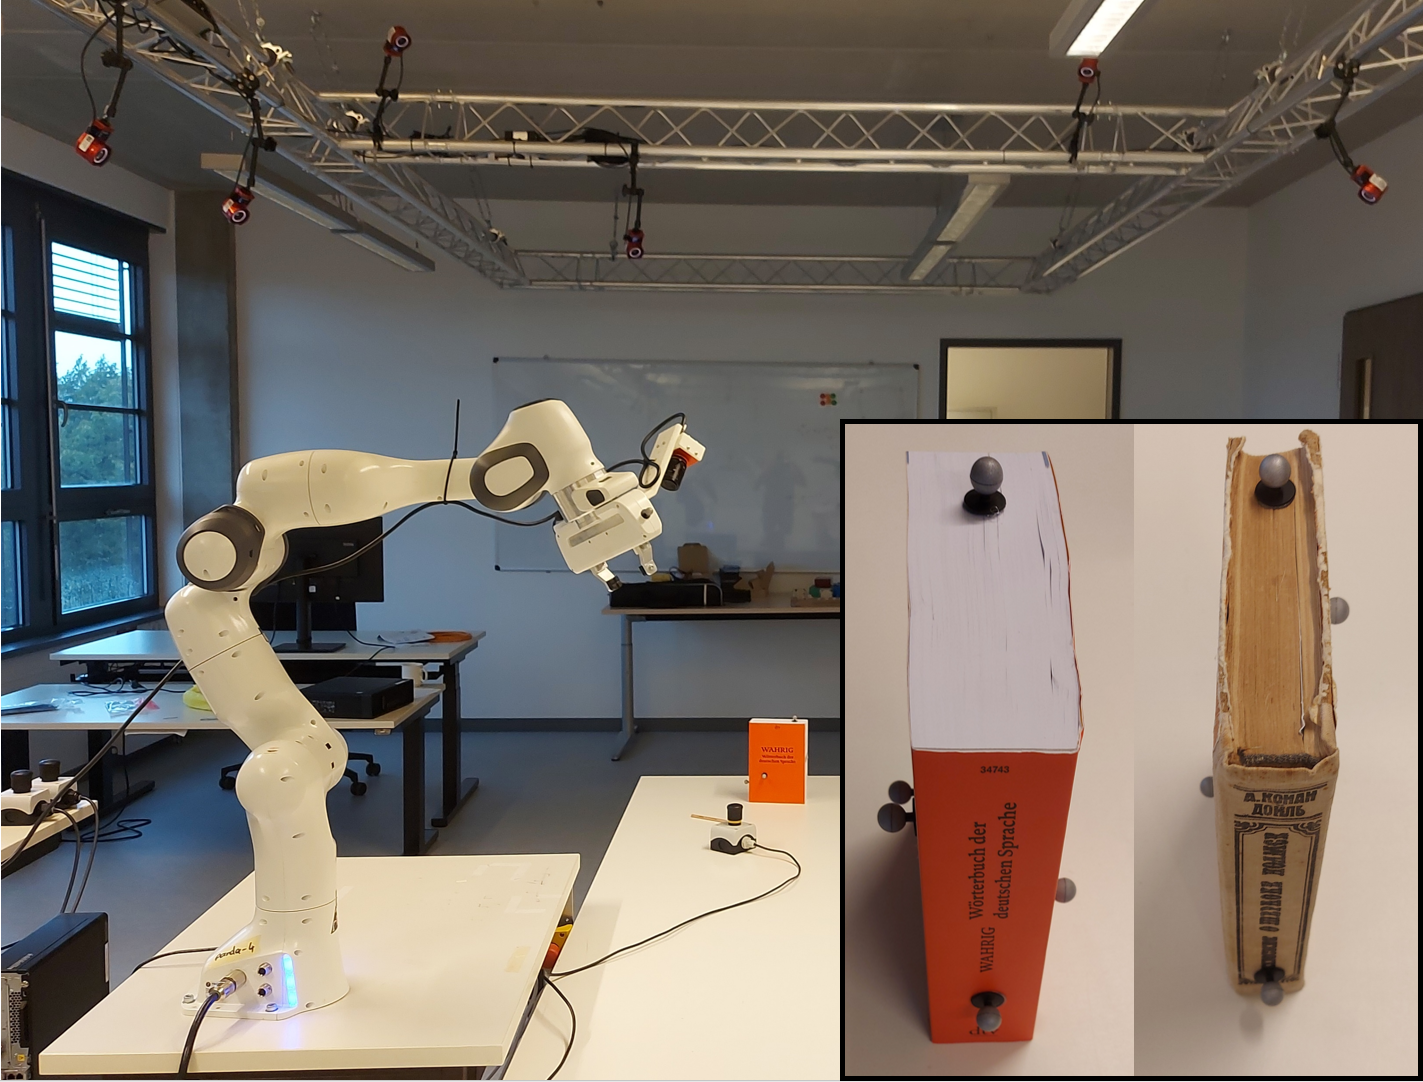
\includegraphics[width=0.9\textwidth]{resources/images/optitrack_setup}
    \caption{Experiment Setup including OptiTrack cameras and objects with markers.}\label{fig:optitrack}
\end{figure}

The recorded data is quite similar to Set 2, just changing the background, having more elements in this new set, and including the information received from the OptiTrack. Concretely, the pose of the gripper and the grasped object are tracked. With that, we can analyze the relative pose of the object with respect to the gripper and detect if slip occurred.\\

Again sequences with and without slip have been recorded for two books, with 5 repetitions for each scenario.\\

For the first book, as shown in ~\Cref{fig:set3_case1}, only a slight rotation is produced towards the end, whereas in \Cref{fig:set3_case2}, there is a slip in the beginning, then it stops and slips again in the opposite direction.\\

In the case of the second book, a similar behavior is observed, with nearly no slip in \Cref{fig:set3_case3} and slip in \Cref{fig:set3_case4}.

\begin{figure}[H]
    \centering
    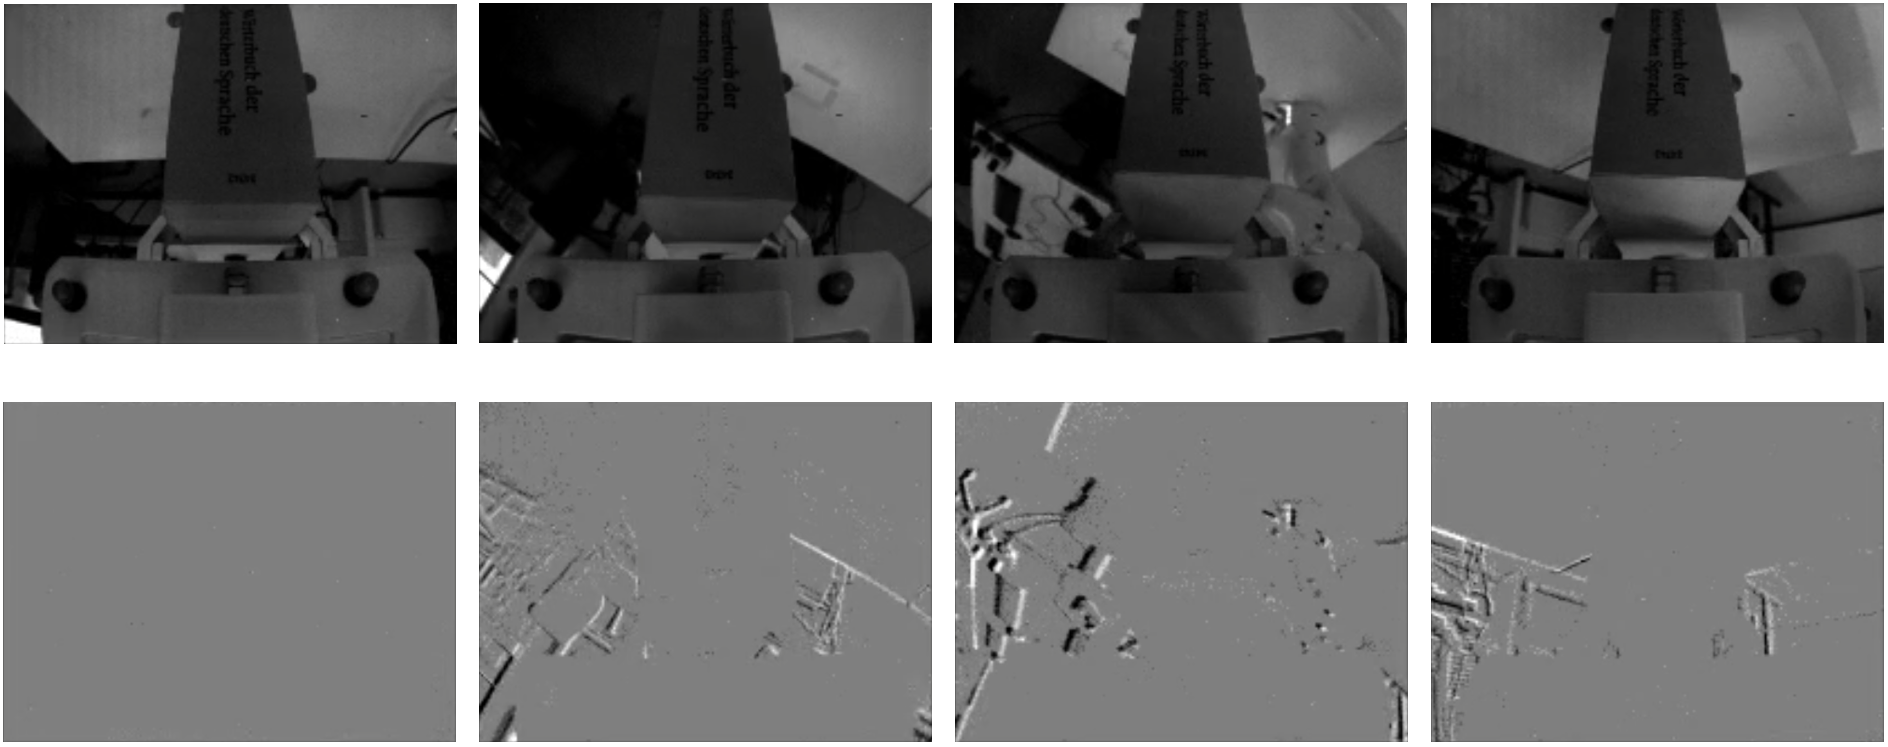
\includegraphics[width=\textwidth]{resources/images/set3_case1}
    \caption{Sequence of grayscale frames (first row) and event images (second row) during no slip, while executing a pick-and-place motion with book no. 1.}\label{fig:set3_case1}
\end{figure}

\begin{figure}[H]
    \centering
    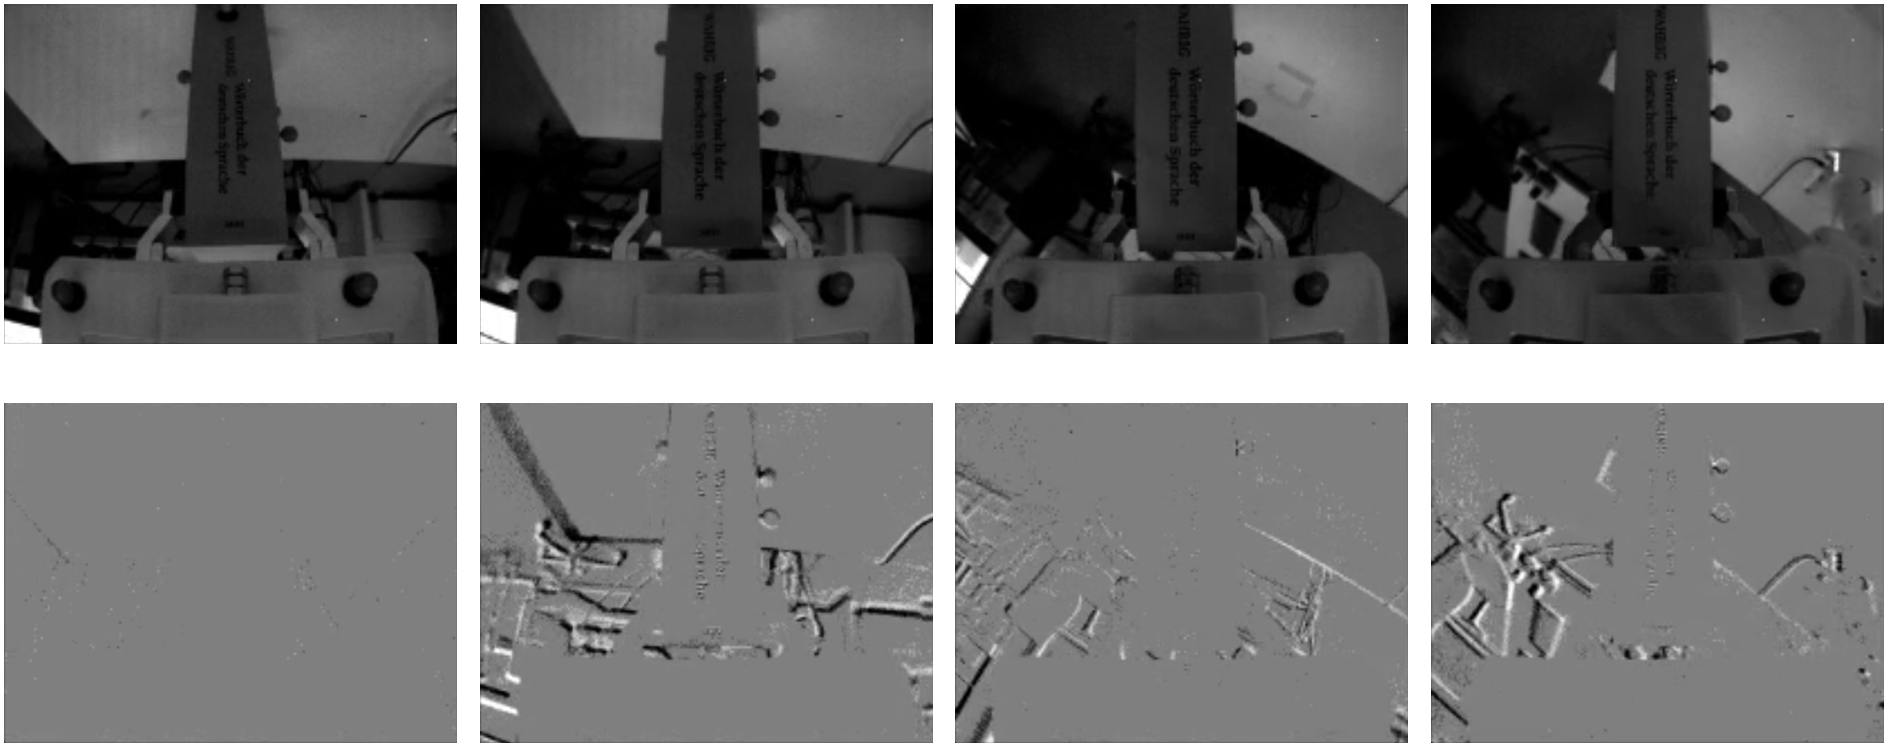
\includegraphics[width=\textwidth]{resources/images/set3_case2}
    \caption{Sequence of grayscale frames (first row) and event images (second row) during a significant slip, while executing a pick-and-place motion with book no. 1.}\label{fig:set3_case2}
\end{figure}

\begin{figure}[H]
    \centering
    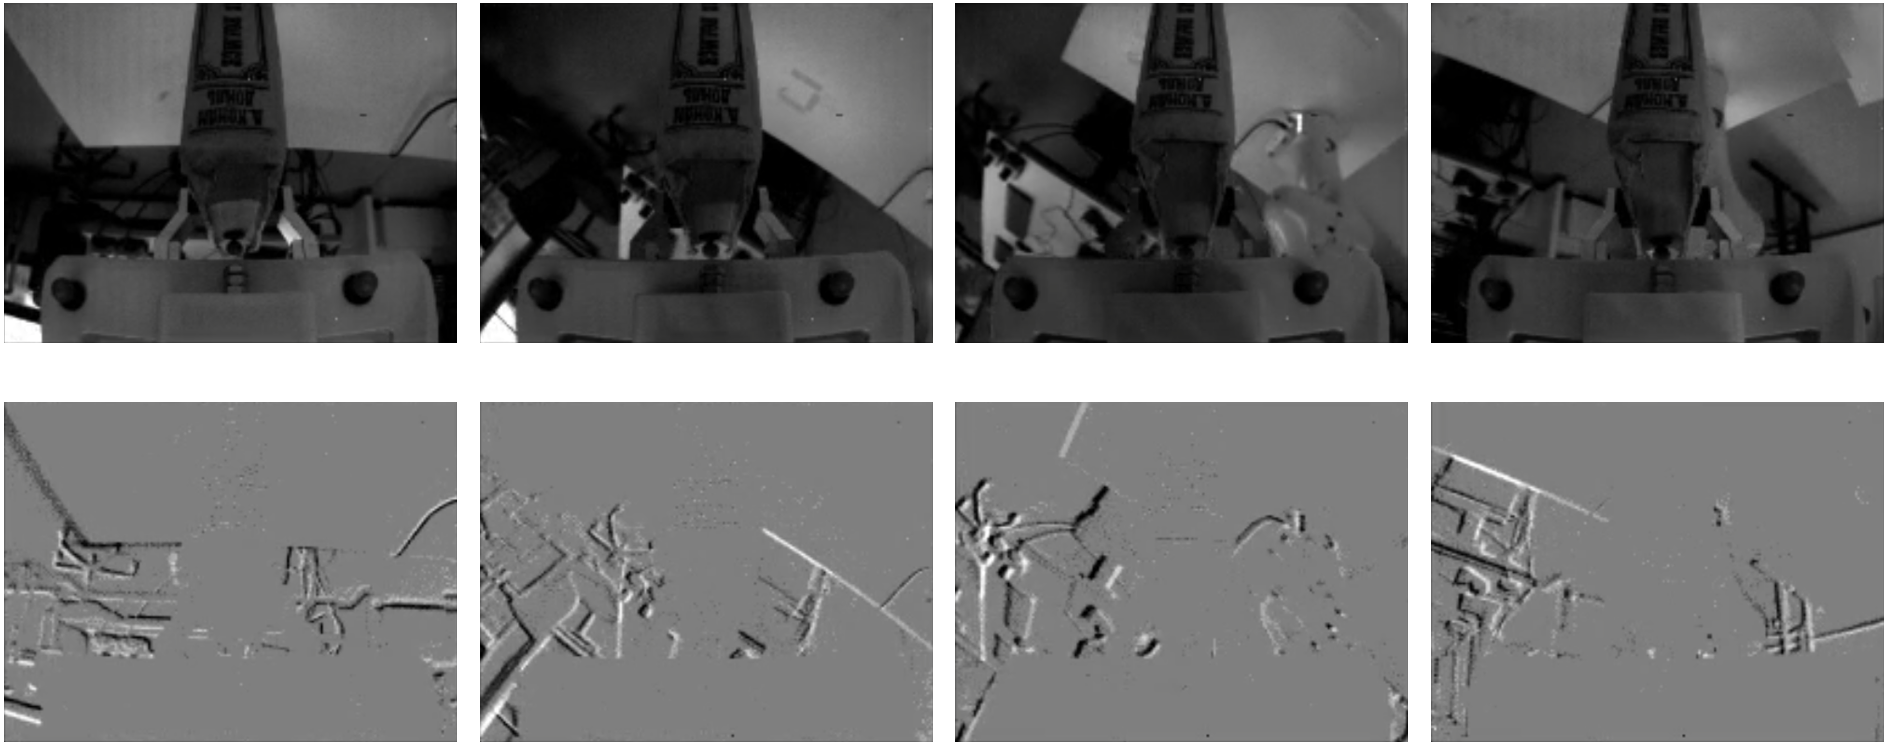
\includegraphics[width=\textwidth]{resources/images/set3_case3}
    \caption{Sequence of grayscale frames (first row) and event images (second row) during a significant slip, while executing a pick-and-place motion with book no. 2.}\label{fig:set3_case3}
\end{figure}

\begin{figure}[H]
    \centering
    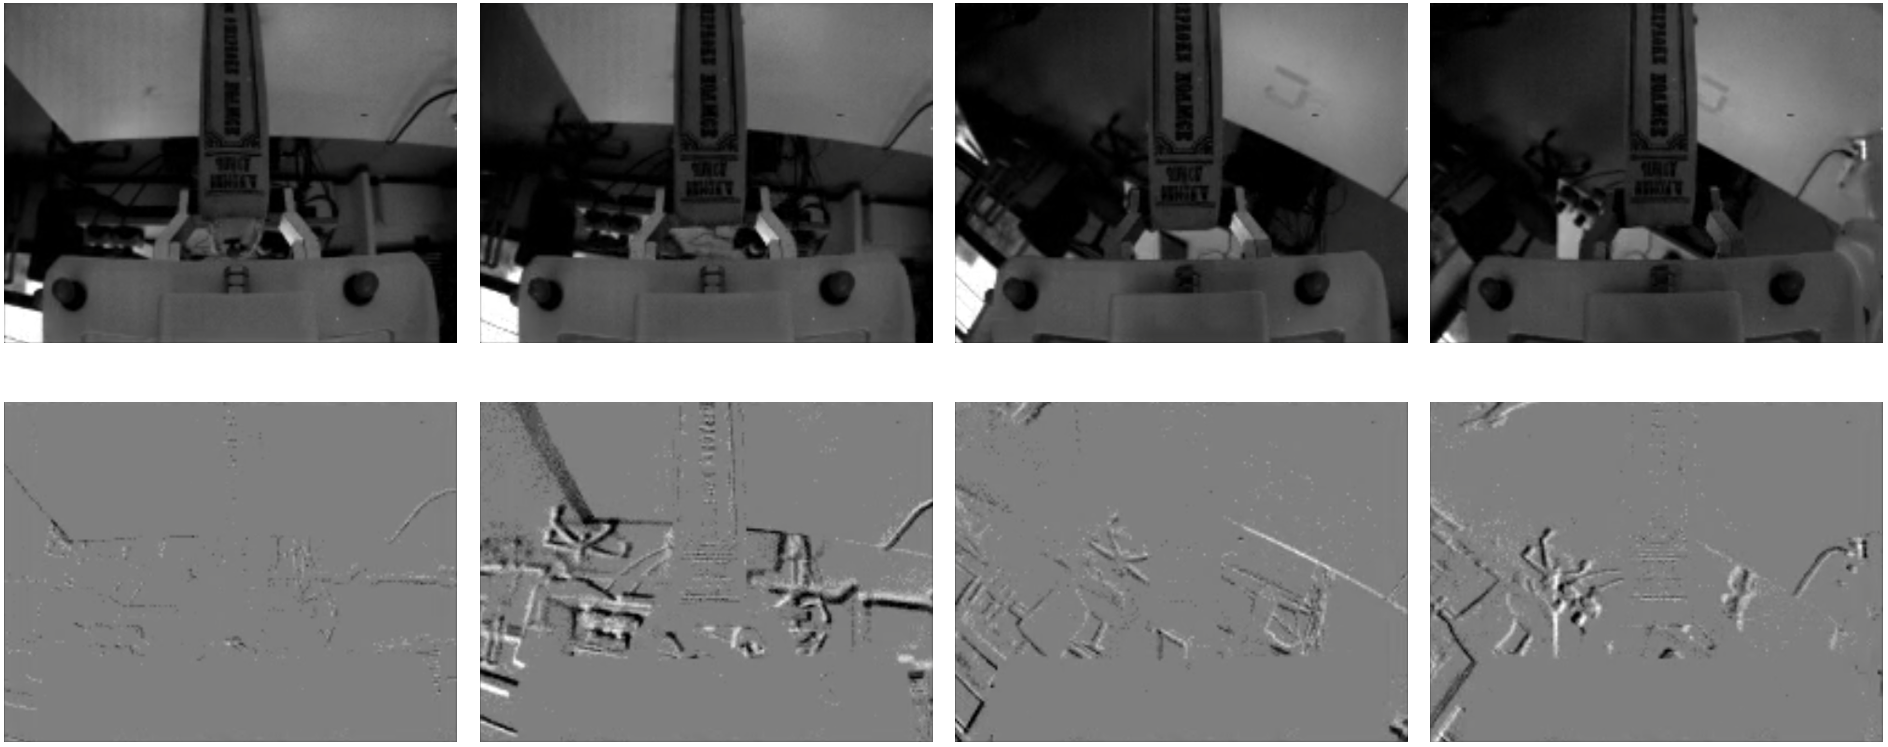
\includegraphics[width=\textwidth]{resources/images/set3_case4}
    \caption{Sequence of grayscale frames (first row) and event images (second row) during no slip, while executing a pick-and-place motion with book no. 2.}\label{fig:set3_case4}
\end{figure}

\section{Conclusion}

In this chapter, all the recorded data is described, the gathering of which was done iteratively, after analyzing the data and determining the new needs after each step. Therefore, these sets of data are meant to help to explore different methods to detect slip and do not make up a final dataset, which should include many more sequences and objects.\\

The next chapter includes the description of the different methods tested to determine slip cases and the discussion of their results.


